\documentclass{purebook}
\usepackage{fixdif}
\usepackage{tikz}

\usetikzlibrary{shapes.callouts,arrows.meta,calc,shadings}

\title{数学分析笔记}
\author{\href{https://github.com/rogeryoungh}{rogeryoungh}}

\begin{document}
\newcommand{\ee}{\mathrm{e}}
\newcommand{\eps}{\varepsilon}
\newcommand{\vbf}[1]{\boldsymbol{#1}}
\newcommand{\seq}[2]{#1_1,\cdots,#1_#2}

\newcommand{\arcsinh}{\operatorname{arcsinh}}
\newcommand{\arccosh}{\operatorname{arccosh}}
\newcommand{\arctanh}{\operatorname{arctanh}}

\maketitle

\frontmatter

\tableofcontents

\mainmatter

%% \newcommand{\dom}{\operatorname{\mathbf{Dom}}}
%% \newcommand{\im}{\operatorname{\mathbf{Im}}}
%% \newcommand{\graph}{\operatorname{\mathbf{graph}}}
%% \newcommand{\LIM}{\operatorname{{LIM}}}

\chapter{实数集与函数}

我初次用的书是华师的数分,现在发觉基础部分有相当多的细节。后参考自李逸的《基本分析讲义》。

若无额外说明,皆在 $\mathbb{R}$ 下。仍有很多术语不曾了解。

\section{前言}

实数理论确实很难以理解。

我初次接触华师数分时,实数看的云里雾里,不知道为什么要罗列一大堆定理,索性直接跳过,读的倒也算通顺。初入门径后,又读了几本其他的书,才感觉到实数理论的意义;但是感觉公理又多又乱,在脑子里缠起来了。继续读下去,观点再高了一点,终于敢说懂了一点。

我尝试讲一讲。按照 Bourbaki 的观点,序结构连同拓扑和代数结构一道组成了数学结构的三大母体。具体的说,如果只有一个光秃秃的集合,我们做不了太多事情。为了在这个集合上展开进一步的讨论,我们需要对它装备一些结构:
\footnote{\href{https://www.zhihu.com/question/47999353/answer/1012530744}{知乎:如何理解数学中的序结构,代数结构和拓扑结构?}}

1. 序结构:元素和元素的排序,比如实数上的大小关系、集合的包含关系。

2. 代数结构:元素和元素的运算,比如加法和乘法。

3. 拓扑结构:子集和子集之间的关系,比如点集的邻近性、敛散性、连续性。

学习实数,主要是抓住这三个方面的性质。接触了更多具体的例子,会对抽象的定义有更多的感悟。

\section{集合和映射}

集合的交并补是熟知的。

定义有序对为 $(a,b) \coloneqq  \{\{a\},\{a,b\}\}$,其中 $a$ 称为有序对的第一坐标,而 $b$ 称为第二坐标。特殊的,$(a,a) = \{a\}$。

定义集合的笛卡尔 Cartesian 乘积为
\[ A \times B \coloneqq  \{(a,b) \mid a\in A \text{且} b\in B\}\]
一般 $A \times B \ne B \times A$。同样可以推广到多个集合
\[ \prod X_i \coloneqq  X_1 \times X_2 \times \cdots \times X_n = (X_1 \times \cdots \times X_{n-1}) \times X_n\]
其元素 $x$ 是多层嵌套,我们可以简记为
\[ x = (\cdots(x_1,x_2),x_3),\cdots,x_n) = (x_1,\cdots,x_n)\]
称 $x_i \coloneqq  \mathrm{pr}_i(x)$ 为 $x$ 的第 $i$ 个分量,$\mathrm{pr}$ 是投影映射。当所有 $X_i$ 都等于 $X$ 时,上述乘积记为 $X^n$。

设 $C$ 和 $D$ 为两个给定的集合。

\begin{definition}[赋值法则]
	设 $R$ 是 $C\times D$ 的一个子集,若满足当 $(c,d_1)\in R$ 且 $(c,d_2)\in R \Rightarrow d_1=d_2$,称 $R$ 是一个赋值法则。
\end{definition}

赋值法则的定义域 Domain 和像域 Image Set 约定如下
\[ \begin{aligned}
		\dom(R) \coloneqq  \{c\in C \mid \exists d \in D, (c,d) \in R\} \\
		\im(R) \coloneqq  \{d\in D \mid \exists c \in C, (c,d) \in R\}  \\
	\end{aligned} \]

\begin{definition}
	设 $R$ 为一个赋值法则,$B$ 为满足 $\im(R) \subseteq B$ 的一个集合,记二元对 $(R,B)$ 为一个映射,$B$ 称为值域。定义 $f$ 的定义域 $A$ 和像域为 $R$ 的定义域和像域。记作
	\[ f:A\to B, a\mapsto f(a) \]
\end{definition}

称 $f$ 的图为
\[ \graph(f) \coloneqq  \{(a,f(a)) \in A\times B \mid a \in A\}\]

对任意给定的 $A$ 的子集 $A_0$,定义 $f$ 在 $A_0$ 上的限制为映射
\[ f \mid_{A_0} = f : A_0 \to B\]

称映射 $f$ 和 $g$ 的复合为
\[ g\circ f: A \to C, a \mapsto g(f(a))\]
显然 $g \circ f$ 仅当 $\im(f) \subseteq \dom(g)$ 时有定义。$f\circ g$ 一般与 $g \circ f$ 不相等。

\begin{itemize}
	\item 若映射 $f$ 满足 $f(a_1) = f(a_2) \Rightarrow a_1,a_2$,称 $f$ 为单射。
	\item 若映射 $f$ 满足对任意的 $b\in B$ 存在 $a\in A$ 满足 $f(a)=b$,称 $f$ 为满射。
	\item 若映射 $f$ 满足$f$ 既是单射又是满射,称 $f$ 为双射。
\end{itemize}

若 $f$ 为双射,我们定义它的逆映射 $f^{-1}$ 为
\[ f^{-1}(b) =  a \Leftrightarrow f(a) = b\]

映射 $\ast: X\times X \to X$ 通常也称为集合 $X$ 上的运算,此时我们把 $\ast(x,y)$ 记做 $x \ast y$。对 $X$ 中的非空子集定义
\[ A \ast B \coloneqq  \ast(a\times B) = \{A \ast b \mid a \in A, b\in B\}\]

如果映射定义中的 $B$ 是一个数域,则把映射称为函数。

\section{序关系}

称集合 $S\times S$ 的子集 $\odot$ 为关系。把 $(x,y) \in \odot$ 记作 $x \odot y$。

\begin{definition}[等价关系]
	若集合 $S$ 上的关系 $\simeq$ 满足

	\begin{itemize}
		\item 自反性:对任意的 $x\in S$ 有 $x \simeq x$。

		\item 对称性:若 $x \simeq y$ 则 $y \simeq x$。

		\item 传递性:若 $x \simeq y$ 且 $y \simeq z$ 则 $x \simeq z$。
	\end{itemize}

	则称 $\simeq$ 为等价关系,一般记作 $\sim$ 或 $=$。
\end{definition}

记 $x\in A$ 的等价类:
\[ [x] \coloneqq  \{y \in A \mid y \sim x\}\]

\begin{definition}[全序关系]
	若集合 $S$ 上的关系 $\preceq$ 满足

	\begin{itemize}
		\item 反对称性:若 $x \preceq y$ 且 $y \preceq x$ 则 $x = y$。

		\item 传递性:若 $x \preceq y$ 且 $y \preceq z$ 则 $x \preceq z$。

		\item 完全性:对任意的 $x,y\in S$ 要么 $x \preceq y$ 要么 $y \preceq x$。(注意蕴含了自反性 $x \preceq x$)。
	\end{itemize}
	则称 $\preceq$ 为全序关系, $(S,\preceq)$ 为全序集。一般用 $\leqslant$ 来表示全序关系.
\end{definition}

对于每一非严格的全序关系 $\leqslant$,定义其对应的严格全序关系 $<$ 为:$a < b$ 等价于 $a \leqslant b$ 且 $a \neq b$。我们对四个关系 $<, \leqslant, >, \geqslant$ 都可以定义全序集。

\begin{definition}
	设全序集 $S' \subseteq S$,若 $x \in S$ 是:

	\begin{itemize}
		\item $S$ 的最大元:若不存在 $y \in S$ 使得 $x < y$,则称 $x$ 是最大元。

		\item $S'$ 的上界:若对于任取的 $x' \in S'$ 满足 $x' \leqslant x$,则称 $x$ 是 $S'$ 的上界。

		\item $S'$ 的上确界:对于任取的 $S'$ 的上界 $y$ 都有 $x \leqslant y$,且 $x$ 是 $S'$ 的上界,则称 $x$ 是 $S'$ 的上确界。
	\end{itemize}
\end{definition}

类似的可定义全序集的最小元、下界、下确界。上、下确界分别记作 $\sup S'$ 和 $\inf S'$。比如取 $A = A' = (0, 1)$,其上下确界都不存在。若取 $A = \mathbb{R}$,上下确界存在也不一定在 $A'$ 里面。

\begin{definition}[最小上界性]
	如果集合 $S$ 的任何非空有上界子集 $S'$ 有最小上界,则称 $S$ 有最小上界性。

	换句话说,若任取非空子集 $S' \subseteq S$,若 $S'$ 在 $S$ 内存在上界,那么 $S'$ 在 $S$ 内存在上确界。
\end{definition}



例如 $\mathbb{Q} \cap (0,\sqrt2)$ 是 $\mathbb{Q}$ 的非空子集,其上界 $\sqrt2$ 并不在 $\mathbb{Q}$ 内。

同样的有最小下界性。可以证明,有最小上界性的一定有最大下界性。展开描述即

\begin{theorem}
	设 $B$ 是具有最小上界性的集合 $S$ 的子集,则对任意的有下界的 $B$ 都有 $\inf B \in S$。
\end{theorem}

\begin{proof}
	对于每个 $B$,构造 $L$ 为 $B$ 的下界组成的集合,显然每个 $B$ 中的元素都是 $L$ 的上界。由最小上界性知,存在 $\sup L \in S$。

	尝试证明 $\inf B=\sup L$。

	对于任意的 $x\in B$,若 $x<\sup L$,则存在比 $\sup L$ 小的 $L$ 的上界 $x$,矛盾。故 $x \geqslant \sup L$,即 $\sup L$ 是 $B$ 的下界。

	设 $B$ 的下界 $x$ 有 $x>\sup L$,那么 $x\in L$,则存在比 $\sup L$ 大的 $L$ 元素,矛盾。故不存在比 $\sup L$ 大的 $B$ 的下界。

	综上,$B$ 的下界存在且 $\inf B=\sup L \in S$。
\end{proof}

\section{代数初步}

首先给出一些性质。

\begin{definition}
	给定集合 $A$,设元素 $x, y, z \in A$,定义如下性质

	\begin{itemize}
		\item 封闭性:若 $A \ast A \subseteq A$,则称 $A$ 在运算 $\ast$ 下封闭。

		\item 结合性:若 $x \ast (y \ast z) = (x \ast y) \ast z$,则称运算 $\ast$ 是结合的。

		\item 交换性:若 $x \ast y = y \ast x$,则称运算 $\ast$ 是交换的。

		\item 单位元(幺元):若存在 $e \in A$ 使得 $e \ast x = x \ast e = x$,则称 $e$ 为 $A$ 上的单位元。

		\item 逆元(么元):若存在 $x^{-1} \in A$ 使得 $x \ast x^{-1} = x^{-1} \ast x = e$,则称 $x^{-1}$ 为 $x$ 在 $A$ 上的逆元。
	\end{itemize}

\end{definition}

注意 $-x$ 和 $x^{-1}$ 只是记号,不代表我们定义出了减法和除法运算。

\begin{definition}[群,半群]
	给定集合 $G$ 和其上的二元运算 $\ast: G \times G \to G$,若:

	\begin{itemize}
		\item 满足结合律,称为半群。

		\item 满足单位元、交换性的半群,称为幺半群、交换半群。

		\item 每个元素都可逆的幺半群,称为群。

		\item 满足交换律的群,称为交换群(Abelian 群)。
	\end{itemize}
\end{definition}

\begin{example}
	群中单位元和逆元唯一。
\end{example}

\begin{proof}
	设 $x$ 存在两个逆元 $y_1, y_2$,有
	\[ y_1 = y_1 \ast e = y_1 \ast x \ast y_2 = e \ast y_2 = y_2 \]
	类似的,设存在两个单位元 $e_1, e_2$,有
	\[ e_1 = e_1 \ast e_2 = e_2 \]
\end{proof}

\begin{definition}[环,域]
	给定集合 $R$ 和其上的二元运算 $(R, +, \ast)$,若:

	\begin{itemize}
		\item 满足 $(R, +)$ 是交换群,$(R, \ast)$ 是幺半群,且乘法关于加法满足分配率,称为环。

		\item 环 $R$ 中 $(R, \ast)$ 可交换,称为交换环。

		\item 除零元外皆可逆的环,称为除环。

		\item 交换除环称为域。
	\end{itemize}
\end{definition}

\section{拓扑初步}

可以想象开集的基为开区间,闭集的基为闭区间。

\begin{definition}[拓扑空间]
	设 $\mathcal{T}$ 是集合 $X$ 子集的集族:

	(O1) 若 $\varnothing \in \mathcal{T}$ 且 $X \in \mathcal{T}$。

	(O2) 若有限个 $U_i \in \mathcal{T}$,则 $\bigcap U_i \in \mathcal{T}$。

	(O3) 若任意个 $U_\alpha \in \mathcal{T}$,则 $\bigcup {U_\alpha} \in \mathcal{T}$。

	则称 $(X, \mathcal{T})$ 为拓扑空间,其中 $\mathcal{T}$ 是此空间的拓扑,$\mathcal{T}$ 的元素称为开集。在无歧义的情况下,也称 $X$ 是拓扑空间。
\end{definition}

\begin{definition}[邻域]
	对于空间 $X$ 和空间内一点 $x \in X$

	1. 若子集 $U$ 包含着某一开集且开集包含着 $x$,则称 $U$ 为 $x$ 的邻域。

	2. 若子集 $U$ 是开集且 $x \in U$,则称 $U$ 为 $x$ 的开邻域。
\end{definition}

\begin{definition}[闭集]
	对于空间 $X$,若其子集 $F$ 满足 $X-F$ 是开集,则称 $F$ 是闭集。
\end{definition}

\begin{example}
	换句话说:

	1. 任意多开集的交集还是开集,有限个开集的并集还是开集。

	2. 任意多闭集的交集还是闭集,有限个闭集的并集还是闭集。
\end{example}

\begin{definition}[闭包,内核]
	设空间 $X$ 和其子集 $A$,记

	1. 所有包含 $A$ 的闭集的交为 $A$ 的闭包 $\overline{A}$,即包含 $A$ 的最小闭集,其中的元素称为 $A$ 的接触点。

	2. 所有包含 $A$ 的开集的并为 $A$ 的内核 $A^{\circ}$,即包含 $A$ 的最大开集。
\end{definition}

\begin{definition}
	对于空间 $X$ 和其子集 $A$,若

	1. $\overline{A} = X$ 则称集合 $A$ 稠密于空间 $X$。

	2. $(\overline{A})^{\circ} = \varnothing$ 则称集合 $A$ 疏(无处稠密)于空间 $X$。
\end{definition}

显然 $\mathbb{N}$ 和 $\mathbb{Z}$ 疏于 $\mathbb{R}$,$\mathbb{Q}$ 和 $\mathbb{R} - \mathbb{Q}$ 稠密于 $\mathbb{R}$。

虽然我们在小学二年级学过无理数的存在性,但我们仍对 $\mathbb{Q}$ 和 $\mathbb{R}$ 性状上的具体区别知之甚少。

\begin{definition}[连通]
	若拓扑空间 $X$ 不能表示为两个不相交闭集的并,则称 $X$ 是连通空间。其子集 $X'$ 若是连通空间,则称 $X'$ 是连通的。
\end{definition}

可以得到 $\mathbb{R}$ 是连通的,$\mathbb{Q}$ 是不连通的。

依定义,闭区间是 $\mathbb{R}$ 内的开集,其任意数量的交都是闭集。假想一个不断变小的区间列,一层套一层。

\begin{definition}[闭区间套]
	给定有限的一列闭区间 $\{ I_i = [a_i, b_i] \}$,若

	(1) 其是下降的
	\[ I_1 \supseteq I_2  \supseteq I_3  \supset \cdots \];

	(2) 区间长度 $\lim\limits_{n \to \infty} (b_i - a_i) = 0$;

	那么称这一列区间是闭缩区间套,简称区间套。
\end{definition}

\begin{definition}[有序域]
	若域 $F$ 是满足如下条件的有序集

	(1) 当 $x,y,z\in F$ 且 $y<z$ 时,$x+y<x+z$。

	(2) 如果 $x,y\in F$,且 $x>0,y>0$,则 $xy>0$。

	那么称 $F$ 是一个有序域。
\end{definition}

例如 $\mathbb{Q}$ 是有序域。

\begin{theorem}[存在定理]
	具有最小上界性的有序域 $\mathbb{R}$ 存在,且包容着 $\mathbb{Q}$ 作为子域。
\end{theorem}

这个命题的证明较为复杂,是从 $\mathbb{Q}$ 出发构造 $\mathbb{R}$,而且其中有很多重要的信息,决定单独一章,这里略过。

\begin{theorem}[Achimedes 原理]
	对于 $x,y \in \mathbb{R}$ 且 $x>0$,那么必定存在正整数 $n$,使得 $nx>y$。
\end{theorem}
\begin{proof}
	设 $A = \{nx \mid n \in \mathbb{N}^+ \}$,若不存在 $n$ 则 $y$ 将是 $A$ 的一个上界,由最小上界性可知 $A$ 的上确界存在。

	又因为小于上确界的数 $\sup A-x$ 不是上确界,即存在 $m\in \mathbb{N}^+$ 使得 $\sup A -x <mx$,即 $\sup A < (m+1)x$,矛盾。

	故必定存在 $n$ 使得 $nx>y$。
\end{proof}

\begin{definition}[度量空间]
	称集合 $X$ 的元素为点,若存在 $X$ 上双变量的函数 $d:X \times X \to \mathbb{R}$,满足($x,y,z\in R$)

	\begin{itemize}
		\item 若 $x\ne y$,则 $d(x,y)$;仅 $d(x,x)=0$。

		\item 对于任意的 $x,y$ 都有 $d(x,y) = d(y,x)$。

		\item 对于任意的 $z$,都有 $d(x,y) \leqslant d(x,z) + d(z,y)$。
	\end{itemize}

	就称 $(X,d)$ 是一个度量空间(度量空间),函数 $d$ 称作其上的距离函数。
\end{definition}

这里的空间的含义是线性空间。

对于 $X$ 的子集 $Y$,定义其距离函数
\[ d_Y: Y \times Y \to \mathbb{R}, (y_1,y_2) \mapsto d_Y(y_1,y_2)=d(y_1,y_2)\]
则 $(Y,d_Y)$ 仍是度量空间,称 $d_Y$ 是 $d$ 在 $Y$ 上的诱导度量。$(Y,d_Y)$ 称作是 $(X,d)$ 的子(度量)空间。

\begin{definition}[稠密性]
	给定度量空间 $(X,d)$,$Y$ 是 $X$ 的子集。如果对任意的 $x\in X$ 和任意小的 $\eps>0$,都存在 $y\in Y$,使得 $d(y,x)<\eps$,我们就称 $Y$ 在 $X$ 中是稠密的。
\end{definition}

\begin{example}
	$\mathbb{Q}$ 在 $\mathbb{R}$ 中稠密:对于 $x,y \in \mathbb{R}$ 且 $x<y$,那么必定存在 $p\in\mathbb{Q}$,使得 $x<p<y$。
\end{example}
\begin{proof}
	由 Achimedes 原理,可设存在 $n\in \mathbb{N}^+$ 使得 $n(y-x)>1$。

	再设存在 $m_1,m_2\in \mathbb{N}^+$,使得 $m_1>nx,m_2>-nx$。于是
	\[ -m_2<nx<m_1 \]
	因此存在 $m\in \mathbb{N}^+$ 有 $-m_2\leqslant m \leqslant m_1$ 使得
	\[ m-1\leqslant nx < m \leqslant 1+nx < ny \]
	从而存在 $p=m/n$ 使得 $x<p<y$。
\end{proof}


\section{数系的构造}

直到我读了陶哲轩的《实分析》时,才感到接受了实数理论。实数的定义是公理化的,不是构造性的。

更具体的说,我们不需要知道实数是什么,只需知道这些对象有什么性质,我们就可以抽象的处理它们。从其他的数学对象出发来构造实数是可能的,有多种多样的模型,只要它们服从所有的公理并正确的运作,都是满足的。

实数究竟有多少性质?从自然数开始。

\begin{axiom}[Peano 公理]
	若集合 $N$ 和其上的映射 $v(n)$ 满足

	(1) $0\in N$。

	(2) 若 $n\in N$,则 $v(n) \in N$。

	(3) 对于任意的 $n\in N$,$v(n) \ne 0$。

	(4) 若 $v(m) \ne v(n)$,则 $m\ne n$。

	(5) 【归纳原理】设 $P(n)$ 是关于自然数的性质,假设只要 $P(n)$ 为真,则 $P(v(n))$ 也为真;且 $P(0)$ 为真。那么对 $N$ 中所有的元素 $P$ 都为真。

	那么称 $N$ 为自然数,记作 $\mathbb{N}$,$v(n)$ 称为后继函数。
\end{axiom}

\subsection{自然数}

设 $m,n\in \mathbb{N}$,定义 $\mathbb{N}$ 上的加法 $+$ 和乘法 $\cdot$ 为
\[
	\begin{aligned}
		0+m\coloneqq m      & ,\quad v(n)+m\coloneqq v(n+m)             \\
		0\cdot m\coloneqq m & ,\quad v(n)\cdot m\coloneqq n \cdot m + m
	\end{aligned}
\]

我们可以利用归纳原理推出我们熟悉的一些性质。

\begin{theorem}[$\mathbb{N}$ 的代数算律]
	对于 $a,b,c\in \mathbb{N}$ 有

	(1) 加法是结合的和交换的,且有单位元 $0$。

	(2) 乘法是结合的和交换的,且有单位元 $1$。

	(3) 分配律:$(a+b) \cdot  c = a \cdot c + b\cdot c$。
\end{theorem}

\begin{definition}[$\mathbb{N}$ 的序]
	设 $m,n\in \mathbb{N}$。

	(1) 若存在 $a\in \mathbb{N}$,使得 $n=m+a$,称 $m$ 小于等于 $n$,记作 $m \leqslant n$。

	(2) 若 $n\geqslant m$ 且 $n\ne m$,则称 $m$ 严格小于 $n$,记作 $m < n$。
\end{definition}

可以验证,$<$ 和 $\leqslant$ 是 $\mathbb{N}$ 上的序关系。

\begin{theorem}[加法保序]
	对于 $a,b\in \mathbb{N}$,若 $a>b$,则 $a+c>b+c$。
\end{theorem}

\subsection{整数}

接下来几节,都是记 $a,b,c$ 为当前集合的元素,$x,y,z$ 都是被构造的集合的元素。

为了表达整数,定义二元组 $(a,b)$,其中 $a,b \in \mathbb{N}$。记全体二元组的集合为 $Z$。我们约定
\[ (a,b) = (c,d) \Leftrightarrow a+d=b+c\]
因为自然数的序是已定义的,于是定义 $Z$ 上的序关系
\[ (a,b) \leqslant (c,d) \Leftrightarrow a+d \leqslant b+c\]
然后是定义 $N$ 上的加法和乘法
\[
	\begin{aligned}
		(a,b) + (c,d)     & \coloneqq  (a+c,b+d) \\
		(a,b) \cdot (c,d) & \coloneqq  (a c,b d)
	\end{aligned}
\]

可以验证,$(n,0)$ 与 $n$ 有相同的性状,我们可以令其相等,从而把自然数嵌入到整数内。至此,我们可以着手验证整数是否满足我们预想的性质。

\begin{theorem}[$\mathbb{Z}$ 的代数算律]
	对于 $x,y,z\in \mathbb{Z}$ 有

	(1) 加法是结合的和交换的,且有单位元 $0$,逆元存在。

	(2) 乘法是结合的和交换的,且有单位元 $1$。

	(3) 分配律:$(x+y) \cdot  z = x \cdot z + y\cdot z$。
\end{theorem}

即 $\mathbb{Z}$ 是一个交换环。于是

\begin{theorem}[$\mathbb{Z}$ 是有序域]
	(1) 加法保序:当 $x,y,z\in \mathbb{Z}$ 且 $y<z$ 时,$x+y<x+z$。

	(2) 乘法保序:如果 $x,y\in \mathbb{Z}$,且 $x>0,y>0$,则 $xy>0$。
\end{theorem}

我们有理由相信,$(a,b)$ 符合我们对整数的一切想象。因此 $Z = \mathbb{Z}$。

另外的,定义整数的负运算为 $-(a,b) = (b,a)$,以此定义减法
\[ x - y \coloneqq  x + (-y)\]
可以验证
\[ (a,0) - (b,0) = (a,b) = a - b\]

\subsection{有理数}

类似的,记整数的二元组 $(a,b)$,其中 $a,b\in \mathbb{Z},b\ne 0$,记全体二元组的集合为 $Q$。我们约定
\[ (a,b) = (c,d) \Leftrightarrow ad = bc\]
因为整数的序是已定义的,于是定义 $Q$ 上的序关系
\[ (a,b) \leqslant (c,d) \Leftrightarrow ad \leqslant bc\]
于是定义 $Q$ 上的加法和乘法
\[
	\begin{aligned}
		(a,b) + (c,d)     & \coloneqq  (ad+bc,b+d)           \\
		(a,b) \cdot (c,d) & \coloneqq  (a \cdot c,b \cdot d) \\
	\end{aligned}
\]
定义加法逆元为 $-(a,b) \coloneqq  (-a,b)$。可以验证,$(a,1)$ 与 $a$ 有相同的性状,我们可以令其相等,从而把整数嵌入到有理数内。

至此,我们可以着手验证有理数是否满足我们预想的性质。

\begin{theorem}[$\mathbb{Q}$ 的代数算律]
	对于 $x,y,z\in \mathbb{Q}$ 有

	(1) 加法是结合的和交换的,且有单位元 $0$,逆元存在。

	(2) 乘法是结合的和交换的,且有单位元 $1$,非零元逆元存在。

	(3) 分配律:$(x+y) \cdot  z = x \cdot z + y\cdot z$。
\end{theorem}

即 $\mathbb{Q}$ 是一个域。

\begin{theorem}[$\mathbb{Q}$ 是有序域]
	(1) 加法保序:当 $x,y,z\in \mathbb{Q}$ 且 $y<z$ 时,$x+y<x+z$。

	(2) 乘法保序:如果 $x,y\in \mathbb{Q}$,且 $x>0,y>0$,则 $xy>0$。
\end{theorem}

我们有理由相信,$(a,b)$ 符合我们对有理数的一切想象。因此 $Q = \mathbb{Q}$。

另外,定义倒数 $(a,b)^{-1} = (b,a)$,显然 $a,b\ne 0$。从而定义除法
\[ x/y \coloneqq  x \cdot y^{-1}\]
可以验证,
\[ (a,1)/(b,1) = (a,b) = a/b\]

\subsection{实数\ ·\ Dedekind 分割}



\begin{definition}[Dedekind 分割]
	对于给定的空间 $S$, $A \subset S, A' = \complement_S A$,若满足以下三个条件

	(D1) $A \ne \varnothing, A \neq S(A' \ne \varnothing)$;

	(D2) 当 $p\in A,q \in A'$ 时,$p<q$;

	(D3) 不存在最大数:任给 $p \in A$,存在 $q \in A$,使得 $p<q$;

	则称 $A$ 为 $S$ 的一个分割。
\end{definition}

直观的来说,我们把整个 $S$ 划分成了下组 $A$ 和上组 $A'$。

记 $\mathbb{Q}$ 上 Dedekind 分割的全体为 $R$,集合的相等即是 $R$ 上的等价关系,$R$ 上的序关系定义是
\[ A \subseteq B \Leftrightarrow A\leqslant B \]
定义加法
\[ A+B \coloneqq  \{ a+b \mid a\in A,b\in B\} \]
于是可以定义负运算
\[ \begin{aligned}
		-A & \coloneqq  \{ s \in \mathbb{Q} \mid \exists r>0,-s-r\in \complement_\mathbb{Q} A\} \\
		-A & \coloneqq  \{ s \in \mathbb{Q} \mid \exists r\in \complement_\mathbb{Q} A,s < -r\}
	\end{aligned} \]


然而乘法因为负数的问题,我们需要分类讨论。$R$ 中存在加法单位元 $0^* = \{x \in \mathbb{Q} \mid x \geqslant 0\}$,对于正实数 $A,B\geqslant 0^*$,定义乘法
\[ A \cdot B \coloneqq  \{ p \in \mathbb{Q} \mid \text{存在}\ 0<a\in A,\ \text{存在}\ 0<b\in B, p<ab\}\]
同时
\[
	A \cdot B \coloneqq \begin{cases}
		-((-A) \cdot B),    & A<0^*, B\geqslant 0^* \\
		-(A \cdot (-B)),    & A\geqslant 0^*, B<0^* \\
		-((-A) \cdot (-B)), & A<0^*, B<0^*          \\
	\end{cases}
\]

当 $A > 0^*$ 时,定义乘法逆元
\[ A^{-1} \coloneqq  \{s \in \mathbb{Q} \mid \exists r \in \complement_\mathbb{Q} A, s < r^{-1}\}\]
当 $A < 0^*$ 时,定义乘法逆元为 $A^{-1} \coloneqq  -(-A^{-1})$。

至此,我们可以着手验证实数是否满足我们预想的性质。

\begin{theorem}[$\mathbb{R}$ 的代数算律]
	对于 $x,y,z\in \mathbb{R}$ 有

	(1) 加法是结合的和交换的,且有单位元 $0$,逆元存在。

	(2) 乘法是结合的和交换的,且有单位元 $1$,非零元逆元存在。

	(3) 分配律:$(x+y) \cdot  z = x \cdot z + y\cdot z$。
\end{theorem}

即 $\mathbb{R}$ 是一个域。

\begin{theorem}[$\mathbb{R}$ 是有序域]
	(1) 加法保序:当 $x,y,z\in \mathbb{R}$ 且 $y<z$ 时,$x+y<x+z$。

	(2) 乘法保序:如果 $x,y\in \mathbb{R}$,且 $x>0,y>0$,则 $xy>0$。
\end{theorem}

我们有理由相信,$\LIM(a_n)$ 符合我们对实数性质的一切想象,从而 $R = \mathbb{R}$。

\begin{theorem}[Dedekind 原理]
	设 $A$ 为 $\mathbb{R}$ 上的 Dedekind 分割,$A' = \complement_\mathbb{R} A$,对于任给的 $a\in A,a' \in A'$,存在 $r \in \mathbb{R}$ 使得 $a < r \leqslant a'$。
\end{theorem}

\begin{proof}
	由于 $a, a'$ 也是 $\mathbb{Q}$ 上的分割,下面使用集合的语言。显然 $a' \in A'$ 是 $A$ 的一个上界。构造
	\[ b = \bigcup_{a \in A} a \]
	下证 $a \subset b \subseteq a'$。

	首先证明 $b$ 是 $\mathbb{Q}$ 上分割。

	\begin{itemize}
		\item D1:显然 $b$ 非空,又因为对于任意的 $a \in A, a' \in A'$ 都有 $a \subset a'$,故 $b \subseteq a'$(注意可取等),即 $b \neq \mathbb{Q}$。
		\item D2:接下来取 $\beta \in b, \beta' \in \complement_\mathbb{Q} b$,于是存在 $a_0 \in A$ 使得 $\beta \in a_0$,此时 $\beta' \notin a_0$ 即 $\beta' \in a_0'$,故 $\beta < \beta'$。
		\item D3:对于任意的 $\beta_1 \in b$,存在 $a_0 \in b$ 使得 $\beta_1 \in a_0$,此时存在 $\alpha_1 \in a_0$ 使得 $\beta_1 < \alpha_1$ 且 $\alpha_1 \in b$。
	\end{itemize}


	接下来证明 $b \notin A$。假设 $b \in A$ 即存在 $a_0$ 使得 $b = a_0$,但由 D3 总是存在 $b = a_0 \subset a_1$,与 $b$ 是全体并集矛盾。

	因此 $b \in A'$,故 $a \subset b \subseteq a'$。
\end{proof}

实数和有理数的最基本的一个区别就是有最小上界性。

\begin{theorem}[确界原理]
	$\mathbb{R}$ 具有最小上界性。即对于 $\mathbb{R}$ 的任何子集 $S$,若 $S$ 在 $\mathbb{R}$ 内存在上界,那么 $S$ 在 $\mathbb{R}$ 内存在上确界。
\end{theorem}
\begin{proof}
	设 $B'$ 是 $S$ 全体上界组成的集合,即 $B' = \{x \mid\forall s \in S, x \geqslant s \}$,令
	\[ B = \complement_\mathbb{R} B' = \{ x \mid \exists s \in S, x < s\} \]
	试证 $B$ 是 $\mathbb{R}$ 的一个分割。D1 和 D2 比较显然。显然对于任意的 $b \in B$ 存在 $s \in S$ 使得 $x < s$,那么总是可以取 $b_2 = \frac{b+s}{2} \in B$ 使 $x < b_2$。

	由上文所证的 Dedekind 原理知,总存在 $u \in \mathbb{R}(B')$ 使得任取上确界 $b' \in B'$ 使得 $u \leqslant b'$,故 $u$ 是上确界。
\end{proof}

\subsection{实数\ ·\ Cauchy 序列}

我们试图得到实数,是因为有理数还不足以表示所有的数,比如 $x^2=2$ 的解。得到实数和前面的方法有所不同,要复杂的多。

一个有理数上的序列 $\{a_n\}$,是一个从集合 $\mathbb{N}$ 到 $\mathbb{Q}$ 的一个映射,即我们以前说的数列。

对于 $\mathbb{Q}$ 上的无限序列 $\{a_n\}$,若对于任意的 $\eps > 0$ 存在 $N \geqslant 0$ 使得当 $j,k \geqslant N$ 时有
\[ d(a_j,a_k) < \eps\]
则称序列 $\{a_n\}$ 为 Cauchy 序列,记作 $\LIM(a_n)$。记 Cauchy 序列的全体为集合 $R$。

对于 Cauchy 序列 $\LIM(a_n),\LIM(b_n)$,若对于任意的 $\eps > 0$ 存在 $N \geqslant 0$ 使得当 $n \geqslant N$ 时有
\[ d(a_n,b_n) < \eps\]
则记作 $\LIM(a_n) = \LIM(b_n)$。

定义 $R$ 的序关系,对于实数 $x,y$,若存在 Cauchy 序列满足 $x=\LIM(a_n),y=\LIM(b_n)$,对于 $n\geqslant 1$ 有 $a_n \leqslant b_n$,则 $\LIM(a_n) \leqslant \LIM(b_n)$。

于是定义 $R$ 上的加法和乘法
\[ \begin{aligned}
		\LIM(a_n) + \LIM(b_n)     & \coloneqq  \LIM(a_n+b_n) & \\
		\LIM(a_n) \cdot \LIM(b_n) & \coloneqq  \LIM(a_nb_n)    \\
	\end{aligned} \]
定义负运算 $-\LIM(a_n) \coloneqq  \LIM(-a_n)$。

定义倒数时会因为恼人的 $0$ 出现了一些困难,解决的方法即是把 $0$ 排出。若存在 $c\in \mathbb{Q}$ 满足 $c > 0$ 使得 $d(a_n,0) \geqslant c$,则称 $\{a_n\}$ 为限制离开零的序列。若 $x$ 为不为零的实数,则必存在一个限制离开零的 Cauchy 序列 $\LIM(a_n) = x$。

于是我们可以定义,设 $x$ 为一个不为零的实数,则存在限制离开零的 Cauchy 序列 $x=\LIM(a_n)$,定义倒数为
\[ x^{-1} \coloneqq  \LIM(a_n^{-1})\]

可以验证,常数 Cauchy 序列 $\{a_n\}$ 与 $a$ 具有相同的性状,因此可以令它们相等,从而使有理数嵌入到实数中。

至此,我们可以着手验证实数是否满足我们预想的性质,在 Dedekind 分割中提过了,这里不再重复。

另外,定义 $R$ 上的 Cauchy 序列,若对于任意的实数 $\eps > 0$ 存在 $N \geqslant 0$ 使得当 $j,k \geqslant N$ 时有
\[ d(a_j,a_k) \leqslant \eps\]

可以证明,$R$ 上的 Cauchy 序列与 $\mathbb{Q}$ 上的 Cauchy 序列等价。

若存在实数 $L$ 满足,存在 $N>0$ 使得当 $n \geqslant N$ 时,都有 $d(a_n,L) \leqslant \eps$,则 $a_n$ 收敛于 $L$,记作
\[ \lim_{n\to \infty} a_n = L\]

可以验证
\[ \LIM(a_n) = \lim_{n\to \infty} a_n\]

\subsection{复数}

记实数的二元组 $(a,b)$,其中 $a,b\in R$,记全体二元组的集合为 $C$。我们约定
\[(a,b) = (c,d) \Leftrightarrow a=b \land  c=d\]
复数没有序关系。定义 $C$ 上的加法和乘法
\[\begin{aligned}
		(a,b) + (c,d)     & \coloneqq  (a+c,b+d)     \\
		(a,b) \cdot (c,d) & \coloneqq  (ac-bd,ad+bc)
	\end{aligned}\]

定义加法逆元为 $-(a,b) \coloneqq  (-a,-b)$。可以验证,$(a,0)$ 与 $a$ 具相同的性状,我们可以令其相等,从而把实数嵌入到复数域内。

定义非零数的乘法逆元 $(a,b)^{-1} \coloneqq  \left(\frac{a}{a^2+b^2},-\frac{b}{a^2+b^2}\right)$。

\section{实数的完备性}

如上所见,实数可以有多种完全不同的定义。换句话说我们可以承认一些公理,使得些都是等价的公理,以下举出几个例子。

\begin{itemize}
	\item R0 Dedekind 原理;
	\item R1 确界原理;
	\item R2 单调有界原理;
	\item R3 区间套原理;
	\item R4 有限覆盖原理;
	\item R5 聚点原理;
	\item R6 致密性原理;
	\item R7 柯西收敛原理;
	\item R8 介值定理;
	\item R9 连通性原理;
	\item R10 Achimedes 原理;
\end{itemize}

这些定理是彼此等价的,其逻辑关系是
\[ \mathrm{R0} \Leftrightarrow \mathrm{R1} \Leftrightarrow\mathrm{R2} \Leftrightarrow\mathrm{R3} + \mathrm{R10} \Leftrightarrow\mathrm{R4} \Leftrightarrow\mathrm{R5} \Leftrightarrow\mathrm{R6} \Leftrightarrow\mathrm{R7}+\mathrm{R10} \Leftrightarrow\mathrm{R8} \Leftrightarrow\text{R9}  \]
因此都可以选作实数的完备性(连续性)公理。互相推导很适合作为课后练习,可以查看 \href{https://zhuanlan.zhihu.com/p/48859870}{实数的完备性定理 - 知乎}。

确界原理由于其简明的性质,我们将在其上构建极限与收敛的体系。







%\subsection{数集·确界原理}
%
%区间分为无限区间和有限区间。
%
%设实数 $a<b$,则称数集 $\{x \mid a<x<b\}$ 为开区间,记作 $(a,b)$;数集 $\{x \mid a\leqslant x \leqslant b\}$ 称为闭区间,记作 $[a,b]$;数集 $\{x \mid a\leqslant x<b\}$ 和 $\{x \mid a < x \leqslant b\}$ 都称为半开半闭区间,分别记作 $[a,b)$ 和 $(a,b]$。以上几类区间统称为有限区间。
%
%满足关系式 $x\geqslant a$ 的全体实数 $x$ 的集合记作 $[a,+\infty)$,类似地,有 $(-\infty,a],(a,\infty),(-\infty,a)$。特殊地 $\mathbb{R} = (-\infty,+\infty)$。这几类区间统称为无限区间。
%
%设 $\delta > 0$,满足 $|x-a|<\delta$ 的 $x$ 的集合称为点 $a$ 的 $\delta$ 邻域,记作 $U(a;\delta)$,或简单的记作 $U(a)$,即有
%$$U(a;\delta) = (a-\delta,a+\delta)\]
%点 $a$ 的空心 $\delta$ 邻域定义为
%$$U^\circ (a;\delta) = \{x \mid 0<|x-a|<\delta\}\]
%也可以简单的记作 $U^\circ(a)$。
%
%此外,常用的邻域还有:
%
%点 $a$ 的 $\delta$ 右邻域 $U_+(a;\delta) = [a,a+\delta)$,左邻域 $U_-(a;\delta)$。以及点 $a$ 的空心 $\delta$ 左、右邻域 $U_{-}^\circ(a)$ 与 $U_{+}^{\circ}(a)$。
%
%以及 $\infty$ 邻域 $U(\infty) = \{x \mid |x|>M\}$,其中 $M$ 为充分大的正数。类似的还有 $U(+\infty) = \{x \mid x>M\}$ 和 $U(-\infty) = \{x \mid x<-M\}$。
%
%\begin{definition}[有界集]
%	设 $S$ 为一个非空数集,若存在数 $M\in$ 使得 $\forall x\in S$
%	
%	(1) 都有 $x\leqslant M$,则称 $M$ 是 $S$ 的一个上界。
%	
%	(2) 都有 $x\geqslant M$,则称 $M$ 是 $S$ 的一个下界。
%\end{definition}
%
%若数集 $S$ 既有上界又有下界,则称 $S$ 为有界集,反之称为无界集。
%
%\begin{theorem}[确界原理]
%	设 $S$ 为非空数集,若 $S$ 有上界,则 $S$ 必有上确界;若 $S$ 有下界,则 $S$ 必有下确界。
%\end{theorem}
%
%若把 $\pm \infty$ 看作非正常上下确界,前文定义视为正常上(下)确界,那么任一非空数集必有上下确界。
%
%\section{函数的上下界}
%
%\begin{definition}
%	设 $f$ 为定义在 $D$ 上的函数。若存在数 $M(L)$,使得对每一个 $x\in D$,有 $f(x)\leqslant M(f(x) \ge L)$,则称 $f$ 为 $D$ 上的有上(下)界函数,$M(L)$ 称为 $f$ 在 $D$ 上的一个上(下)界。
%
%	反之,若存在数 $M(L)$,使得对每一个 $x\in D$,有 $f(x) \geqslant M(f(x) \leqslant L)$,则称 $f$ 为 $D$ 上的有无上(下)界函数。
%\end{definition}
%
%\begin{definition}
%	设 $f$ 为定义在 $D$ 上的函数。若存在正数 $M$,使得对每一个 $x\in D$,有 $|f(x)|\leqslant M$,则称 $f$ 为 $D$ 上的有界函数。
%
%	反之,若存在正数 $M$,使得对每一个 $x\in D$,有 $|f(x)|\ge M$,则称 $f$ 为 $D$ 上的无界函数。
%\end{definition}
%
%记函数 $f$ 在 $D$ 上的上确界为 $\sup_{x\in D} f(x)$,类似的有 $\inf_{x\in D} f(x)$。
%
%\begin{definition}
%	设 $f$ 为定义在 $D$ 上的函数,若对任何 $x_1,x_2\in D$,当 $x_1<x_2$ 时:
%
%	(1) 总有 $f(x_1) \leqslant f(x_2)$,则称 $f$ 为 $D$ 上的增函数,若成立严格不等式 $f(x_1) < f(x_2)$ 时,称 $f$ 为 $D$ 上的严格增函数。
%
%	(2) 总有 $f(x_1) \geqslant f(x_2)$,则称 $f$ 为 $D$ 上的减函数,若成立严格不等式 $f(x_1) > f(x_2)$ 时,称 $f$ 为 $D$ 上的严格减函数。
%\end{definition}
%
%增函数和减函数统称为单调函数,严格增函数和严格减函数统称为严格单调函数。
%
%严格单调函数必有反函数,其也为严格单调函数。
%
%\begin{definition}
%	设 $D$ 为对称于原点的数集, 函数 $f$ 为定义在 $D$ 上的函数。若对每一个 $x\in D$:
%
%	(1) 有 $f(-x) = -f(x)$,则称 $f$ 为 $D$ 上的奇函数。
%
%	(2) 有 $f(-x) = f(x)$,则称 $f$ 为 $D$ 上的偶函数。
%\end{definition}    % 实数集与函数
\chapter{数列极限}

\section{数列极限的概念}

\begin{definition}[数列极限的 $\eps - N$ 定义]
	设 $\{a_n\}$ 为数列,$A$ 为定数。若对任给的正数 $\eps$,总存在正整数 $N=N(\eps)$,使得当 $n>N$ 时有
	\[|a_n - A| < \eps\]
	则称数列 $\{a_n\}$ 收敛于 $A$,或称 $A$ 为数列 $\{a_n\}$ 的极限,记作
	\[\lim\limits_{n\to \infty} a_n = A \text{,或}\ a_n \to a(n \to \infty)\]
\end{definition}

若数列 $\{a_i\}$ 存在 $A \in \mathbb{R}$ 使得 $a_n \to A$ 成立,则称为收敛的。反之称为发散的,逻辑展开即:对任意 $A$ 都有 $a_n$ 不收敛至 $A$。

在使用 $\eps - N$ 语言时,$N(\eps)$ 的选取是非常有技巧的,需要多加练习才能感悟到。

特殊地,若 $\lim\limits_{n\to \infty} a_n = 0$,则称 $\{a_n\}$ 为无穷小数列。

\begin{definition}[无穷大数列]
	若数列 $\{a_n\}$ 满足:对任意正数 $M>0$,存在正整数 $N$,使得当 $n>N$ 时,

	(1) $a_n>M$,则称数列 $\{a_n\}$ 发散于正无穷大,记作 $\lim\limits_{n\to \infty} a_n = +\infty$,或 $a_n \to +\infty$。

	(2) 有 $a_n<M$,则称数列 $\{a_n\}$ 发散于负无穷大,记作 $\lim\limits_{n\to \infty} a_n = -\infty$,或 $a_n \to -\infty$。

	两者合称无穷大数列。
\end{definition}

\begin{example}
	证明数列 $a_n = \sin n$ 发散。
\end{example}

\begin{proof}
	不妨假设其极限为 $A$,任取 $\eps$ 存在 $N$ 使得当 $n > N$ 时有 $|\sin n - A| < \eps$。注意到
	\[ |2 \sin 1 \cos n| = |\sin(n+1) - \sin(n-1)| < 2 \eps \]
	可以得到 $\cos n \to 0$,又
	\[ |\sin 2n| = 2 |\sin n \cos n| < 2 |\cos n| < \frac{2\eps}{\sin 1} \]
	从而 $\sin n \to 0$。显然有矛盾
	\[ |\sin^2 2n + \cos^2 2n| < \frac{5 \eps^2}{\sin^2 1} < 1 \]
	故不存在极限,即发散。
\end{proof}

\section{收敛数列的性质}

\begin{theorem}[唯一性]
	若数列 $\{a_n\}$ 收敛,则它只有一个极限。
\end{theorem}

\begin{proof}
	如果数列 $\{a_n\}$ 同时以 $A,B$ 为极限,即任给 $\eps>0$,总存在 $N_1,N_2$,使得
	\[|a_n-A|<\eps,n>N_1;\quad |a_n-B|<\eps,n>N_2\]
	那么当 $n>\max\{N_1,N_2\}$ 时需要恒成立
	\[2\eps > |a_n-A|+|a_n-B| \geqslant |A-B|\]
	当 $A\ne B$ 时,对于 $2\eps <|A-B|$ 不恒成立,因此只能 $A=B$。
\end{proof}

\begin{theorem}[有界性]
	若数列 $\{a_n\}$ 收敛,则 $\{a_n\}$ 有界。
\end{theorem}

\begin{proof}
	不妨设 $\lim\limits_{n\to \infty} a_n = A$。令 $\eps = 1$,那么存在 $n>N$ 使得
	\[|a_n-A| \leqslant 1\]
	令
	\[M = \{|a_1|,\cdots,|a_N|,|A-1|,|A+1|\}\]
	那么对任意正整数 $n$,总有 $|a_n|\leqslant M$。
\end{proof}

\begin{theorem}[保序性]
	设 $\lim\limits_{n\to \infty} a_n = A,\lim\limits_{n\to \infty} b_n = B$,则有

	(1) 如果存在 $N$ 使得当 $n>N$ 时有 $a_n\geqslant b_n$ 恒成立,则 $A\geqslant B$。

	(2) 反之,如果 $A>B$,则存在 $N$ 使得当 $n>N_1$ 时 $a_n>b_n$ 恒成立。
\end{theorem}
\begin{proof}
	(1) 如果设 $B-A=2\delta>0$,那么存在 $N_2,N_3>N$
	\[|a_n-A|<\delta,n>N_2;\qquad |b_n-B|<\delta,n>N_3\]
	于是当 $n>\max\{N_2,N_3\}$ 时有
	\[a_n<A+\delta=B-\delta<b_n\]
	因此矛盾,故 $A\geqslant B$。

	(2) 设 $A-B=2\delta>0$,那么存在 $N_2,N_3$
	\[|a_n-A|<\delta,n>N_2;\qquad |b_n-B|<\delta,n>N_3\]
	于是存在 $N_1=\max\{N_2,N_3\}$,当 $n>N_1$ 时有
	\[a_n>A-\delta=B+\delta>b_n\]
\end{proof}

若 $b_n$ 是常数列,$A\ne 0$,我们还可得到推论:存在 $N$,使得当 $n>N$ 时,有
\[ \frac{1}{2}|A| < |a_n| < \frac{3}{2}|A| \]

\begin{theorem}[迫敛性,夹逼定理]
	设数列 $\{a_n\},\{b_n\},\{c_n\}$ 满足当 $n>N_0$ 有 $a_n\leqslant c_n\leqslant b_n$。若
	\[\lim_{n\to \infty}a_n = A = \lim_{n\to \infty}c_n\]
	则 $\lim\limits_{n\to \infty}b_n = A$。
\end{theorem}
\begin{proof}
	即对于任给的 $\eps>0$,存在 $N_1,N_2$,使得当 $n>N_1$ 有
	\[A-\eps<a_n<A+\eps\]
	当 $n>N_2$ 有
	\[A-\eps<c_n<A+\eps\]
	因此当 $n>\max\{N_0,N_1,N_2\}$ 时,有
	\[A-\eps < a_n \leqslant b_n \leqslant c_n < A+\eps\]
\end{proof}

\begin{example}
	如果 $a_1, \cdots, a_k > 0$,那么有
	\[ \lim_{n \to \infty} \sqrt[n]{a_1^n + \cdots + a_k^n} = \max\{a_1, \cdots, a_k\} \]
\end{example}

\begin{proof}
	不妨设 $a_1 = \max\{a_1, \cdots, a_k\}$,那么有
	\[ a_1 < \sqrt[n]{a_1^n + \cdots + a_k^n} < \sqrt[n]{k a_1^n} \to a_1 \]
	由夹逼原理知原式成立。
\end{proof}

\begin{theorem}[四则运算]
	设 $\lim\limits_{n\to \infty} a_n = A,\lim\limits_{n\to \infty} b_n = B$,则有

	(1) $\{\alpha a_n+\beta b_n\}$ 收敛到 $\alpha A+\beta B$,其中 $\alpha,\beta$ 为常数。

	(2) $\{a_nb_n\}$ 收敛到 $AB$。

	(3) 当 $B\ne 0$ 时,$\{a_n/b_n\}$ 收敛到 $A/B$。
\end{theorem}
\begin{proof}
	(1) 任给 $\eps >0$,存在 $N_1,N_2$ 使得
	\[|a_n-A|<\frac{\eps}{2|\alpha|+1},n>N_1;\qquad |b_n-B|<\frac{\eps}{2|\beta|+1},n>N_2\]
	则当 $n>\max\{N_1,N_2\}$ 时有
	\[
		\begin{aligned}
			|(\alpha a_n+\beta b_n)-(\alpha A+\beta B)| & \leqslant |\alpha||a_n-A|+|\beta||b_n-B|                          \\
			                                            & < \frac{\eps|\alpha|}{2|\alpha|+1}+\frac{\eps|\beta|}{2|\beta|+1} \\
			                                            & < \frac{\eps}2+\frac{\eps}2=\eps
		\end{aligned}
	\]

	(2) 由收敛数列的有界性,存在 $M$ 使得 $|a_n|\leqslant M$,那么
	\[0\leqslant |a_nb_n-AB|=|(a_n-A)b_n+A(b_n-B)|\leqslant M|a_n-A|+|A||b_n-B|\]
	由迫敛性知 $\lim\limits_{n\to \infty}|a_nb_n-AB| =0$。

	(3) 由保号性的推论,存在 $N$ 使得当 $n>N$ 时有 $|b_n|>\dfrac{|B|}{2}$,那么
	\[0 \leqslant \left|\frac{1}{b_n}-\frac{1}{B}\right| = \frac{|b_n-B|}{|b_n||B|} \leqslant \frac{2}{|B|^2}{|b_n-B|}\]
	由迫敛性知 $\lim\limits_{n\to \infty}\left|\frac{1}{b_n}-\frac{1}{B}\right| =0$。
\end{proof}

\subsection{Stolz 定理}

Stolz 定理主要是用来处理 $\infty/\infty$ 型和 $0/0$ 型极限,可以认为是洛必达的替代。

\begin{theorem}
	对于任意的 $1 \leqslant k \leqslant n$,设 $b_k>0$ 且 $m \leqslant \dfrac{a_k}{b_k} \leqslant M$,则有
	\[m \leqslant \frac{\sum a_n}{\sum b_n} \leqslant M\]
\end{theorem}

\begin{theorem}[Stolz 定理一]
	设数列 $\{x_n\},\{y_n\}$,且 $\{y_n\}$ 严格单调地趋于 $+\infty$,如果
	\[\lim_{n\to \infty}\frac{x_n-x_{n-1}}{y_n-y_{n-1}}=A\]
	则
	\[\lim_{n\to \infty} \frac{x_n}{y_n} = A\]
\end{theorem}

\begin{proof}
	分类讨论 Todo……
\end{proof}

\begin{theorem}[Stolz 定理二]
	设数列 $\{y_n\}$ 严格单调地趋于 $0$,且数列 $\{x_n\}$ 也收敛到 $0$,那么如果
	\[\lim_{n\to \infty}\frac{x_n-x_{n-1}}{y_n-y_{n-1}}=A\]
	则
	\[\lim_{n\to \infty} \frac{x_n}{y_n} = A\]
\end{theorem}

\begin{proof}
	分类讨论 Todo……
\end{proof}


\section{数列收敛的判别法则}

我们需要一些更方便的判别法则。

\subsection{单调数列}

若数列 $\{a_n\}$ 各项满足关系式 $a_n \leqslant a_{n+1}(a_n \geqslant a_{n+1})$,则称 $\{a_n\}$ 为递增(递减)数列,统称为单调数列。

\begin{theorem}[单调有界定理]
	单调有界数列必有极限。
\end{theorem}

\begin{proof}
	不妨设 $\{a_i\}$ 为有上界的单调递增序列,由确界原理知存在上确界 $\beta$。按其定义,任给 $\eps > 0$ 都存在 $N$ 使得 $\beta - \eps < a_N < \beta$(否则 $\beta - \eps$ 就是新的上确界)。故 $|a_n - \beta| < \eps$,即收敛至 $\beta$。
\end{proof}

\subsection{子列}

设 $\{a_n\}$ 为数列,如果 $\{n_k\}$ 是一列严格递增的正整数,则数列 $\{a_{n_k}\}$ 称为数列 $\{a_n\}$ 的一个子列。子列显然有性质 $n_k \geqslant k$,归纳易证。

特殊的子列 $\{a_{2k}\}$ 和 $\{a_{2k-1}\}$ 分别称为偶子列与奇子列。数列本身也是其自己的子列。

\begin{theorem}[Weierstrass 致密性定理]
	任何有界数列必定有收敛的子列。
\end{theorem}

\begin{proof}
	不妨设数列包含无数个不同的 $a_n$,否则显然成立。假设数列有界,设其值域为 $[A_0, B_0]$。注意到我们可以对分区间为 $[A_0, \frac{A_0 + B_0}{2}]$ 和 $[\frac{A_0 + B_0}{2}, B_0]$,至少其中之一包含无穷多个 $a_n$,记为 $[A_1, B_1]$。我们可以不断划分,得到一闭缩区间套
	\[ [A_0, B_0] \supset [A_1, B_1] \subset \cdots   \]
	总是可以在区间中找到下标递增的项,即我们要求的子列。
\end{proof}

\begin{theorem}
	数列 $\{a_n\}$ 收敛的充要条件:$\{a_n\}$ 的任何子列都收敛。
\end{theorem}

\subsection{Cauchy 准则}

\begin{definition}
	设 $\{a_n\}$ 为数列,如果任给 $\eps>0$,均存在 $N(\eps)$ 使任取 $m,n>N(\eps)$ 有
	\[|a_m-a_n| < \eps\]
	则称 $\{a_n\}$ 为 Cauchy 数列或基本列。
\end{definition}

反之,若存在 $\eps > 0$ 使得任给 $N$ 都存在 $n, m > N$ 使得
\[ |a_n - a_m| \geqslant \eps \]
则称该数列为非 Cauchy 的。

\begin{theorem}
	Cauchy 数列必定是有界数列。
\end{theorem}
\begin{proof}
	取 $\eps=1$,则存在 $N$ 使得当 $m,n>N$ 时有
	\[|a_m-a_n| < 1\]
	令 $M = \max\{|a_k|+1 \mid 1 \leqslant k \leqslant N+1\}$,则当 $n\leqslant N$ 时显然有 $|a_n|\leqslant M$,而当 $n>N$ 时有
	\[|a_n| \leqslant |a_n-a_{N+1}| + |a_{N+1} < 1+ |a_{N+1}| \leqslant M\]
	这说明 $\{a_n\}$ 是有界数列。
\end{proof}

\begin{theorem}[Cauchy 收敛准则]
	$\{a_n\}$ 为 Cauchy 数列当且仅当它是收敛的。
\end{theorem}
\begin{proof}
	(1) 充分性:设 $\{a_n\}$ 收敛到 $A$,则任给 $\eps >0$ 存在 $N$,当 $n>N$ 时有
	\[|a_n-A|\leqslant \frac{\eps}{2}\]
	因此当 $m,n>N$ 时有
	\[|a_m-a_n| \leqslant |a_m-A| + |A-a_n| < \frac{\eps}{2}+\frac{\eps}{2}=\eps\]
	这说明 $a_n$ 为 Cauchy 数列。

	(2) 必要性:已证 Cauchy 列有界,则必存在收敛子列 $\{a_{u_k}\}$,因此任给 $\eps > 0$ 存在 $N_1$ 使得当 $u_i > N_1$ 时有
	\[ | a_{u_i} - A| < \frac{\eps}{2} \]
	又由定义知存在 $N_2$ 使得任取 $n, m > N_2$ 有
	\[ |a_n - a_m| < \frac{\eps}{2} \]
	因此取 $N = \max\{N_1, N_2\}$,取 $u_k > N$,则当 $n > N$ 时有
	\[ |a_n - A| \leqslant |a_n - a_{u_k}| + | a_{u_k} - A| \leqslant \eps \]
\end{proof}

\begin{theorem}[不动点原理]
	设递推数列 $a_{n+1} = f(a_n)$,假设 $a_n \subset (\alpha, \beta)$,若存在常数 $L \in (0, 1)$ 使得对任意 $x,y \in (\alpha, \beta)$ 有
	\[ |f(x) - f(y)| \leqslant L|x-y| \]
	则数列收敛。
\end{theorem}

\begin{proof}
	首先类似于等比
	\[ |a_{n+1} - a_n| \leqslant \cdots \leqslant L^{n-1}|a_2 - a_1| \]
	从而
	\[ |a_{n+k} - a_{n}| \leqslant \sum_{i=1}^{k} |a_{n + i} - a_{n + i - 1}| \leqslant \sum_{i=1}^{k} L^{n+i} |a_{2} - a_{1}| \leqslant \frac{L^{n-1}}{1-L}|a_2 - a_1|  \]
	由 Cauchy 收敛准则知数列收敛。
\end{proof}

\section{常见数列}

首先我们定义三个数列
\[ a_n = \left(1 + \frac{1}{n}\right)^n, \quad b_n = \left(1 + \frac{1}{n}\right)^{n+1}, e_n = \sum_{i=0}^{n}\frac{1}{k!} \]
我们通常定义 $a_n$ 的极限为 $\ee$。下证三者极限存在且相同。

其中 $e_n$ 的单调性是显然的。我们先证:
\[ a_n < a_{n+1},\quad b_n > b_{n+1} \]
首先
\[ \begin{aligned}
	a_n &= \sum_{k=0}^{n} \binom{n}{k} \frac{1}{n^k} \\
	&= 1 + \sum_{k=1}^n \frac{1}{k!} \prod_{j=1}^{k-1} \left(1 - \frac{j}{n}\right) \\
	&< 1 + \sum_{k=1}^n \frac{1}{k!} \prod_{j=1}^{k-1} \left(1 - \frac{j}{n+1}\right) \\
	&< 1 + \sum_{k=1}^{n+1} \frac{1}{k!} \prod_{j=1}^{k-1} \left(1 - \frac{j}{n+1}\right) = a_{n+1} \\
\end{aligned} \]
再借助 Bernoulli 不等式
\[ \begin{aligned}
	\frac{b_{n-1}}{b_n} &= \frac{\left(1 + \frac{1}{n-1}\right)^n}{\left(1 + \frac{1}{n}\right)^{n+1}} \\
	&= \left(1+\frac{1}{n^2 - 1}\right)^n \frac{1}{1 + \frac{1}{n}} \\
	&> \left(1+\frac{n}{n^2 - 1}\right) \frac{1}{1 + \frac{1}{n}} \\
	&= 1 + \frac{1}{(n+1)^2(n-1)} > 1
\end{aligned} \]

注意到当 $n > 2$ 时
\[ a_n \leqslant 1 + \sum_{k=1}^n \frac{1}{k!} = e_n \leqslant 2 + \sum_{k=2}^n \frac{1}{k(k-1)} = 3 - \frac{1}{n} < 3 \]
故 $a_n$ 和 $b_n$ 单调有界,故必有极限。再注意到
\[ b_n = \left(1 + \frac{1}{n}\right) a_n \]
由极限的四则运算,故 $b_n$ 的极限也存在,且 $a_n$ 和 $b_n$ 收敛于同一个值。

我们定义 $a_n$ 的极限为 $\ee$,下证 $e_n \to \ee$。注意到固定 $u$ 有
\[ \begin{aligned}
	a_n &= 1 + \sum_{k=1}^n \frac{1}{k!} \prod_{j=1}^{k-1} \left(1 - \frac{j}{n}\right) \\
	&> 1 + \sum_{k=1}^u \frac{1}{k!} \prod_{j=1}^{k-1} \left(1 - \frac{j}{n}\right)
\end{aligned} \]
那么令 $n \to \infty$,有
\[ e_k = \sum_{k=0}^u \frac{1}{k!}\leqslant a_n \to \ee \]
故由夹逼定理知 $e_n \to \ee$。

    % 数列极限
\chapter{线性方程组的解系}

\section{\texorpdfstring{$n$ 维向量空间 $K^n$}{n 维向量空间 Kn}}

取定一个数域 $K$,设 $n$ 是任意给定的一个正整数。令
$$K^n=\{(a_1,\cdots,a_n) \mid a_i\in K,i=1,\cdots,n\}$$
如果 $a_1=b_1,\cdots,a_n=b_n$,则称 $K^n$ 中的两个元素:$(a_1,\cdots,a_n),(b_1,\cdots,b_n)$ 相等。

在 $K^n$ 中规定加法运算:
$$(a_1,\cdots,a_n)+(b_1,\cdots,b_n):=(a_1+b_1,\cdots,a_n+b_n)$$

在 $K$ 的元素与 $K^n$ 的元素之间规定数量乘法运算:
$$k(a_1,\cdots,a_n) := (ka_1,\cdots,ka_n)$$

容易验证加法和数量乘法运算满足下述八条运算法则:对于 $\aaa,\bbb,\ggg\in K^n,k,l\in K$ 有

1. $\aaa+\bbb=\bbb+\aaa$

2. $(\aaa+\bbb)+\ggg=\aaa+(\bbb+\ggg)$

3. 把元素 $(0,\cdots,0)$ 记作零元素 $\ling$,使得
$$\ling + \aaa = \aaa + \ling = \aaa$$

4. 对于 $\aaa = (a_1,\cdots,a_n)\in K^n$,定义其负元素
$$-\aaa := (-a_1,\cdots,-a_n)$$
于是有
$$\aaa + (-\aaa) = (-\aaa)+\aaa = 0$$

5. $1\aaa = \aaa$

6. $(kl)\aaa = k(l\aaa)$

7. $(k+l)\aaa = k\aaa + l\aaa$

8. $k (\aaa+\bbb) = k\aaa + k\bbb$

\begin{definition}[$n$ 维向量空间]
	数域 $K$ 上所有 $n$ 元有序数组组成的集合 $K^n$,连同定义在它上面的加法运算和数量乘法运算,及其满足的 8 条运算法则一起,称为数域 $K$ 上的一个 $n$ 维向量空间。$K^n$ 的元素称为 $n$ 维向量;设向量 $\aaa  = (a_1,\cdots,a_n)$,称 $a_i$ 是 $\aaa$ 的第 $i$ 个分量。
\end{definition}

在 $n$ 维向量空间 $K^n$ 中,可以定义减法运算
$$\aaa - \bbb := \aaa + (-\bbb)$$

$n$ 元有序数组写成一行,称为行向量;写成一列,称为列向量,也可以看作行向量的转置。

$K^n$ 可以看成是 $n$ 维行向量组成的向量空间,也可以看作是列向量组成的向量空间。

\begin{definition}[线性组合]
	给定向量组 $\aaa_1,\cdots,\aaa_s$,再任给 $K$ 中的一组数 $k_1,\cdots,k_s$,那么向量
	$$k_1 \aaa_1+\cdots+k_s \aaa_s$$
	称为向量组 $k_1,\cdots,k_s$ 的一个线性组合,其中 $k_1,\cdots,k_s$ 称为系数。
\end{definition}

\begin{definition}[线性表出]
	给定向量组 $\aaa_1,\cdots,\aaa_s$,对于 $\bbb \in K^n$,若存在 $K$ 中的一组数 $k_1,\cdots,k_s$ 满足
	$$\bbb = k_1\aaa_1+\cdots+k_s\aaa_s$$
	那么称 $\bbb$ 可以由向量组 $\aaa_1,\cdots,\aaa_s$ 线性表出。
\end{definition}

于是可以把数域 $K$ 上的 $n$ 元线性方程组

\begin{equation*}
	\left\{
		\begin{matrix}
			a_{11}x_1+a_{12}x_2+\cdots+a_{1n}x_n=b_1\\
			a_{21}x_1+a_{22}x_2+\cdots+a_{2n}x_n=b_2\\
			\cdots\qquad\cdots\qquad\cdots\\
			a_{n1}x_1+a_{n2}x_2+\cdot +a_{nn}x_n=b_n
		\end{matrix}
	\right.
\end{equation*}

写成
$$x_1\aaa_1+\cdots+x_n\aaa_n=\bbb$$
其中 $\aaa_1,\cdots,\aaa_n$ 是线性方程组的列向量组,$\bbb$ 是由常数项组成的列向量。

\begin{definition}[线性子空间]
	$K^n$ 的一个非空子集 $U$ 是 $K^n$ 的一个线性子空间,那么满足
	
	1. $U$ 对于 $K^n$ 的加法封闭:$\aaa,\ggg\in U \Rightarrow \aaa+\ggg \in U$

	2. $U$ 对于 $K^n$ 的乘法封闭:$\aaa \in U,k\in K \Rightarrow k\aaa \in U$
\end{definition}

特殊的,${0}$ 也是 $K^n$ 的一个,称为零子空间。$K^n$ 本身也是 $K^n$ 的一个子空间。

$\aaa_1,\cdots,\aaa_n$ 的所有线性组合也是 $K^n$ 的一个子空间,称为 $\aaa_1,\cdots,\aaa_n$ 生成(张成)的子空间,记作
$$\langle \aaa_1,\cdots,\aaa_n\rangle:=\{k_1\aaa_1+\cdots+k_s\aaa_s \mid k_i\in K,i=1,\cdots,s\}$$

于是线性方程组有解,等价与 $\bbb$ 可以由 $\aaa_1,\cdots,\aaa_n$ 线性表出,即 $\bbb \in \langle\aaa_1,\cdots,\aaa_n\rangle$。




    % 函数极限
\chapter{函数的连续性}

\section{连续性的概念}

\begin{definition}[连续性]
	设函数 $f$ 在某 $U(x_0)$ 上有定义。若
	$$\lim_{x\to x_0}f(x) = f(x_0)$$
	则称 $f$ 在点 $x_0$ 连续。
\end{definition}

记 $\Delta x = x-x_0$,称为自变量 $x$ 在点 $x_0$ 的增量或改变量。设 $y_0=f(x_0)$,相应的函数 $y$ 在点 $x_0$ 的增量记为
$$\Delta y = f(x)-f(x) = f(x+\Delta)-f(x_0) = y-y_0$$ 

连续性的 $\varepsilon-\delta$ 形式定义:若对任给的 $\varepsilon>0$,存在 $\delta>0$,使得当 $|x-x_0|<\delta$ 时,有 $|f(x)-f(x_0)|<\varepsilon$,则称函数 $f$ 在点 $x_0$ 连续。

或者进一步表示为
$$\lim_{x\to x_0}f(x) = f\left(\lim_{x\to x_0}x\right)$$

\begin{definition}
	设函数 $f$ 在某 $U_+(x_0)$ 上有定义。若
	$$\lim_{x\to x_0^+}f(x) = f(x_0)$$
	则称 $f$ 在点 $x_0$ 右连续。同理左连续。
\end{definition}

因此函数 $f$ 在点 $x_0$ 连续的充要条件是:$f$ 在点 $x_0$ 既是左连续,又是右连续。

\begin{definition}[间断点]
	设函数 $f$ 在某 $U^\circ(x_0)$ 上有定义。若 $f$ 在点 $x_0$ 无定义,或 $f$ 在点 $x_0$ 有定义而不连续,则称点 $x_0$ 为函数 $f$ 的间断点或不连续点。
\end{definition}

若 $\displaystyle\lim_{x\to x_0}f(x)=A$,而 $f$ 在点 $x_0$ 无定义,或有定义但 $f(x_0)\ne A$,则称点 $x_0$ 为 $f$ 的可去间断点。

若函数 $f$ 在点 $x_0$ 的左、右极限都存在,但 $\displaystyle\lim_{x\to x_0^+}f(x) \ne \lim_{x\to x_0^-}f(x)$,则称点 $x_0$ 为函数 $f$ 的跳跃间断点。

可去间断点与跳跃间断点统称为第一类间断点,所有其他形式的间断点统称为第二类间断点。

若函数 $f$ 在区间 $I$ 上的每一点都连续,则称 $f$ 为 $I$ 上的连续函数。对于闭区间或半开区间的端点,函数在这些点上连续是指左连续或右连续。

\section{连续函数的性质}

\begin{theorem}[局部有界性]
	若函数 $f$ 在点 $x_0$ 连续,则 $f$ 在某 $U(x_0)$ 上有界。
\end{theorem}

\begin{theorem}[局部保号性]
	若函数 $f$ 在点 $x_0$ 连续,且 $f(x_0)>0$,则对任何正数 $r<f(x_0)$,存在某 $U(x_0)$,使得对一切 $x\in U(x_0)$,有 $f(x)>r$。
\end{theorem}

\begin{theorem}[四则运算]
	若函数 $f,g$ 在点 $x_0$ 连续,则 $f\pm g,f\cdot g,f/g$ 也都在点 $x_0$ 连续。
\end{theorem}

\begin{theorem}
	若函数 $f$ 在点 $x_0$ 连续,$g$ 在点 $u_0$ 连续,$u_0=f(x_0)$,则复合函数 $g\circ f$ 在 $x_0$ 连续。
\end{theorem}

\begin{definition}
	设 $f$ 为定义在数集 $D$ 上的函数。若存在 $x_0\in D$,使得对一切 $x\in D$,有 $f(x_0)\ge f(x)$,则称 $f$ 在 $D$ 上有最大值,并称 $f(x_0)$ 为 $f$ 在 $D$ 上的最大值。
\end{definition}

\begin{theorem}[最大、最小值定理]
	若函数 $f$ 在闭区间 $[a,b]$ 上连续,则 $f$ 在闭区间 $[a,b]$ 上有最大值与最小值。
\end{theorem}

\begin{theorem}[介值定理]
	若函数 $f$ 在闭区间 $[a,b]$ 上连续,且 $f(a)\ne f(b)$。若 $\mu$ 为介于 $f(a)$ 和 $f(b)$ 之间的任何实数。则至少存在一点 $x_0\in (a,b)$ 使得 $f(x_0)=\mu$。
\end{theorem}

\begin{theorem}
	若函数 $f$ 在 $[a,b]$ 上严格单调并连续,则反函数 $f^{-1}$ 在其定义域 $[\min\{f(a),f(b)\},\max\{f(a),f(b)\}]$ 上连续。
\end{theorem}

\begin{definition}
	设 $f$ 是定义在区间 $I$ 上的函数。若对任给的 $\varepsilon>0$,存在 $\delta=\delta(\varepsilon)>0$,使得对任何 $x',x''\in I$,只要 $|x'-x''|<\delta$,就有 $|f(x')-f(x'')|<\varepsilon$,就称函数 $f$ 在去间 $I$ 上一致连续。
\end{definition}

\begin{theorem}[一致连续性]
	若函数 $f$ 在闭区间 $[a,b]$ 上连续,则 $f$ 在 $[a,b]$ 上一致连续。
\end{theorem}

\section{初等函数的连续性}

\begin{theorem}
	设 $p>0$,$a,b$ 为任意两个实数,则有
	$$p^a\cdot p^b = p^{a+b},(p^a)^b=p^{ab}$$
\end{theorem}

\begin{theorem}
	指数函数 $a^x(a>0)$ 在 $\RR$ 上是连续的。
\end{theorem}
    % 导数理论
\chapter{矩阵的相抵与相似}

\section{等价关系与集合的划分}

等价关系还是记录一下。

\begin{definition}
	设 $S$ 是一个非空集合,我们把 $S\times S$ 的一个子集 $W$ 叫做 $S$ 上的一个二元关系。如果 $(a,b)\in W$,那么称 $a$ 与 $b$ 有 $W$ 关系;如果 $(a,b)\notin W$,那么称 $a$ 与 $b$ 没有 $W$ 关系。
\end{definition}

当 $a$ 与 $b$ 有 $W$ 关系时,记作 $aWb$,或 $a\sim b$。

\begin{definition}
	集合 $S$ 上的一个二元关系 $\sim$ 如果具有下述性质:$\forall a,b,c\in S$,有
	
	(1) 反身性 $a\sim a$
	
	(2) 对称性 $a\sim b \Rightarrow b\sim a$
	
	(3) 传递性 $a\sim b$ 且 $b\sim c \Rightarrow a\sim c$
	
	那么称 $\sim$ 是 $S$ 上的一个等价关系。
\end{definition}

\begin{definition}
	设 $\sim$ 是集合 $S$ 上的一个等价关系,$a\in S$ ,令
	\[\overline{a} \coloneqq  \{x\in S \mid x\in a\}\]
	称 $\overline{a}$ 是由 $a$ 确定的等价类,$a$ 称为等价类 $\overline{a}$ 的一个代表。
\end{definition}

\begin{definition}
	如果集合 $S$ 是一些非空子集 $S_i$ ($i\in I$,这里 $I$ 表示指标集)的并集,并且其中不相等的子集一定不相交,那么称集合 $\{S
		_i \mid i\in I\}$ 是 $S$ 的一个划分,记作 $\pi(S)$。
\end{definition}

\begin{theorem}
	设 $\sim$ 是集合 $S$ 上的一个等价关系,则所有等价类组成的集合是 $S$ 的一个划分,记作 $\pi_\sim(S)$。
\end{theorem}

\begin{definition}
	设 $\sim$ 是集合 $S$ 上的一个等价关系。由所有等价类组成的集合称为 $S$ 对于关系 $\sim$ 的商集,记作 $S/\sim$。
\end{definition}

注意,$S$ 的商集 $S/\sim$ 里的元素是 $S$ 的子集,不是 $S$ 的元素。

设 $\sim$ 是集合 $S$ 上的一个等价关系,一种量或一种表达式如果对于同一个等价类里的元素是相等的,那么称这种量或表达式是一个不变量。恰好能完全决定等价类的一组不变量称为完全不变量。

\section{矩阵的相抵}

数域 $K$ 上所有 $s\times n$ 矩阵组成的集合记作 $M_{s\times n}(K)$,当 $s=n$ 时简记为 $M_n(K)$。

\begin{definition}
	对于数域 $K$ 上的 $s\times n$ 矩阵 $A$ 和 $B$,如果从 $A$ 经过一系列初等行变换和初等列变换能变成矩阵 $B$,那么称 $A$ 与 $B$ 是相抵的,记作 $A\overset{\text{相抵}}{\sim}B$。
\end{definition}

相抵是集合 $M_{s\times n}(K)$ 上的一个二元关系,不难验证相抵是一个等价关系,其下矩阵 $A$ 的等价类称为 $A$ 的相抵类。

\begin{theorem}
	设数域 $K$ 上 $s\times n$ 矩阵 $A$ 的秩为 $r$,如果 $r>0$,那么 $A$ 相抵于下述形式的矩阵
	\[\left(\begin{matrix}
				E_r & 0  \\
				0   & 0
			\end{matrix}\right)\]
	称其为 $A$ 的相抵标准形;如果 $r=0$,那么相抵标准形是零矩阵。
\end{theorem}

\begin{theorem}
	数域 $K$ 上 $s\times n$ 矩阵 $A$ 与 $B$ 相抵当且仅当它们的秩相等,即矩阵的秩是相抵关系下的完全不变量。
\end{theorem}

\section{广义逆矩阵}

\begin{theorem}
	设 $A$ 是数域 $K$ 上 $s\times n$ 非零矩阵,则矩阵方程
	\[AXA = A\]
	一定有解。如果 $\rank(A) = r$,并且
	\[A = P\left(\begin{matrix}
				E_r & 0  \\
				0   & 0
			\end{matrix}\right)Q\]
	其中 $P,Q$ 分别是 $K$ 上 $s$ 级、$n$ 级可逆矩阵,那么矩阵方程的通解为
	\[X = Q^{-1}\left(\begin{matrix}
				E_r & B  \\
				C   & D
			\end{matrix}\right)P^{-1}\]
	其中 $B,C,D$ 分别是数域 $K$ 上任意的 $r\times (s-r),(n-r)\times r,(n-r)\times (s-r)$ 矩阵。
\end{theorem}

\begin{definition}
	设 $A$ 是数域 $K$ 上 $s\times n$ 非零矩阵,则矩阵方程 $AXA = A$ 的每一个解都称为 $A$ 的一个广义逆矩阵,简称广义逆。用 $A^-$ 表示。
\end{definition}

\begin{theorem}
	非齐次线性方程组 $AX = \beta$ 有解的充分必要条件是
	\[\beta = AA^-\beta\]
\end{theorem}

\begin{theorem}
	非齐次线性方程组 $AX = \beta$ 有解时,它的通解为
	\[X  = A^-\beta\]
\end{theorem}

\begin{theorem}
	数域 $K$ 上 $n$ 元齐次线性方程组 $AX = 0$ 的通解为
	\[X  = (I_n - A^-A)\vbf{Z}\]
	其中 $A^-$ 是 $A$ 的任意一个广义逆,$\vbf{Z}$ 取遍 $K^n$ 中任意列向量。
\end{theorem}

% \begin{definition}
%	 设 $A$ 是复数域上 $s\times n$ 矩阵,矩阵方程组
%	 \[\begin{cases}
%		 AXA = A,\\
%		 XAX = X,\\
%		 (AX)^* = AX,\\
%		 (XA)^* = XA,
%	 \end{cases}\]
%	 称为 $A$ 的 Penrose 方程组,它的解称为 $A$ 的 Moore-Penrose 广义逆,记作 $A^+$。
% \end{definition}44

\section{矩阵的相似}

\begin{definition}
	设 $A$ 与 $B$ 都是数域 $K$ 上 $n$ 级矩阵,如果存在数域 $K$ 上一个 $n$ 级可逆矩阵 $P$,使得
	\[P^{-1}AP = B\]
	那么称 $A$ 与 $B$ 是相似的,记作 $A\sim B$。
\end{definition}

同样相似是集合 $M_{s\times n}(K)$ 上的一个二元关系,不难验证相似是一个等价关系,其下矩阵 $A$ 的等价类称为 $A$ 的相似类。

相似的矩阵具有相等的行列式和秩。

\begin{definition}
	$n$ 级矩阵 $A=(a_{ij})$ 的主对角线上元素的称为 $A$ 的迹,记作 $\tr(A)$。
\end{definition}

不难验证矩阵的迹都有如下性质
\[
	\begin{aligned}
		\tr(A+B) & = \tr(A) + \tr(B) \\
		\tr(kA)  & = k\tr(A)         \\
		\tr(AB)  & = \tr(BA)
	\end{aligned}
\]

\begin{theorem}
	相似的矩阵都有相同的迹。
\end{theorem}

这表明,矩阵的行列式、秩、迹都是相似关系下的不变量,简称为相似不变量。

如果 $n$ 级矩阵相似于一个对角矩阵,那么称 $A$ 可对角化。

\begin{theorem}
	数域 $K$ 上 $n$ 级矩阵 $A$ 可对角化的充分必要条件是,$K^n$ 中有 $n$ 个线性无关的列向量 $\seq{\alpha}{n}$,以及 $K$ 中有 $n$ 个数 $\seq{\lambda}{n}$(它们之中有些可能相等),使得
	\[A\alpha_i = \lambda_i \alpha_i, i=1,\cdots,n\]
	这时,令 $P = (\seq{\alpha}{n})$,则
	\[P^{-1}AP = \diag\{\seq{\lambda}{n}\}\]
\end{theorem}

\section{矩阵的特征值和特征向量}

\begin{definition}
	设 $A$ 是数域 $K$ 上的一个 $n$ 级矩阵,如果 $K^n$ 中有非零列向量 $\alpha$ 使得
	\[A \alpha = \lambda_0\alpha,\text{且}\ \lambda_0\in K\]
	那么称 $\lambda_0$ 是 $A$ 的一个特征值,称 $\alpha$ 是 $A$ 的属于特征值 $\lambda_0$ 的一个特征向量。
\end{definition}

注意零向量不是特征向量。

\begin{theorem}
	设 $A$ 是数域 $K$ 上的 $n$ 级矩阵,则
	
	(1) $\lambda_0$ 是 $A$ 的一个特征值当且仅当 $\lambda_0$ 是 $A$ 的特征多项式 $|\lambda E-A|$ 在 $K$ 中的一个根。\index{tezhengduoxiangshi@特征多项式}
	
	(2) $\alpha$ 是 $A$ 的属于特征值 $\lambda_0$ 的一个特征向量当且仅当 $\alpha$ 是齐次线性方程组 $(\lambda_0E-A)X = \vbf{0}$  的一个解。
\end{theorem}

设 $\lambda_j$ 是 $A$ 的一个特征值,把齐次线性方程组 $(\lambda_jE-A)X = \vbf{0}$ 的解空间称为 $A$ 的属于 $\lambda_j$ 的特征子空间,其中的全部非零向量都是 $A$ 的属于 $\lambda_j$ 的全部特征向量。

\begin{theorem}
	相似的矩阵有相等的特征多项式。
\end{theorem}

因此矩阵的特征多项式和特征值都是相似不变量。

\begin{definition}
	设 $A$ 是数域 $K$ 上的 $n$ 级矩阵,$\lambda_1$ 是 $A$ 的一个特征值。把 $A$ 的属于 $\lambda_1$ 的特征子空间的维数叫做特征值 $\lambda_1$ 的几何重数,而把 $\lambda_1$ 作为 $A$ 的特征多项式根的重数叫做 $\lambda_1$ 的代数重数。\index{daishuchongshu@代数重数} \index{jihechognshu@几何重数}
\end{definition}

代数重数简称为重数。

\begin{theorem}
	设 $\lambda_1$ 是数域 $K$ 上的 $n$ 级矩阵 $A$ 的一个特征值,则 $\lambda_1$ 的几何重数不超过它的代数重数。
\end{theorem}

\section{矩阵可对角化的条件}

\begin{theorem}
	数域 $K$ 上 $n$ 级矩阵 $A$ 可对角化的充分必要条件是 $A$ 有 $n$ 个线性无关的特征向量 $\seq{\alpha}{n}$,此时令
	\[P=(\seq{\alpha}{n})\]
	则
	\[P^{-1}AP = \diag\{\seq{\lambda}{n}\}\]
	其中 $\lambda_i$ 是 $\alpha_i$ 所属的特征值。上述对角矩阵称为 $A$ 的相似标准形。
\end{theorem}

\begin{theorem}
	设 $\lambda_1,\lambda_2$ 是数域 $K$ 上 $n$ 级矩阵 $A$ 的不同特征值,$\seq{\alpha}{s}$ 与 $\seq{\beta}{r}$ 分别是 $A$ 的属于 $\lambda_1,\lambda_2$ 的线性无关的特征向量,则 $\seq{\alpha}{s},\seq{\beta}{r}$ 线性无关。
\end{theorem}

\begin{theorem}
	设 $\seq{\lambda}{m}$ 是数域 $K$ 上 $n$ 级矩阵 $A$ 的不同特征值,$\alpha_{j1},\cdots,\alpha_{jr_j}$ 是 $A$ 的属于 $\lambda_j$ 的线性无关的特征向量,$j=1,\cdots,m$,则向量组
	\[\alpha_{11},\cdots,\alpha_{1r_1},\cdots,\alpha_{m1},\cdots,\alpha_{1r_m}\]
	线性无关。
\end{theorem}

\begin{theorem}
	数域 $K$ 上 $n$ 级矩阵 $A$ 可对角化的充分必要条件是:$A$ 的特征多项式的全部复根都属于 $K$,并且 $A$ 的每个特征值的几何重数等于它的代数重数。
\end{theorem}

\section{实对称矩阵的对角化}

若对于 $n$ 级矩阵 $A,B$,存在一个 $n$ 级正交矩阵 $T$,使得 $T^{-1}AT=B$,那么称 $A$ 正交相似于 $B$。

\begin{theorem}
	实对称矩阵的特征多项式的每一个复根都是实数,从而它们都是特征值。
\end{theorem}

\begin{theorem}
	实对称矩阵 $A$ 的属于不同特征值的特征向量是正交的。
\end{theorem}

\begin{theorem}
	实对称矩阵一定正交相似于对角矩阵。
\end{theorem}

对于 $n$ 级实对称矩阵 $A$,找一个正交矩阵 $T$,使得 $T^{-1}AT$ 为对角矩阵的步骤如下。

1. 计算 $|\lambda I- A|$,求出它的全部不同的根:$\seq{\lambda}{m}$,它们是 $A$ 的特征值。

2. 对于每一个特征值 $\lambda_j$,求 $(\lambda_jI-A)X = \vbf{0}$ 的一个基础解系 $\alpha_{j1},\cdots,\alpha_{jr_j}$;然后把它们施密特正交化和单位化,得到 $\eta_{j1},\cdots,\eta_{jr_j}$。它们也是 $A$ 的属于 $\lambda_j$ 的一个特征向量。

3. 令
\[T=(\eta_{11},\cdots,\eta_{1r_1},\cdots,\eta_{m1},\cdots,\eta_{mr_m})\]
则 $T$ 是 $n$ 级正交矩阵,且
\[T^{-1}AT = \diag\{\lambda_{1},\cdots,\lambda_{1},\cdots,\lambda_{m},\cdots,\lambda_{m}\}\]
    % 积分理论
%% \newcommand{\ji}[2]{#1_1,\cdots,#1_#2}
%% \newcommand{\transpose}[1]{{#1}^\mathsf{T}}
%% \newcommand{\diag}{\operatorname{diag}}

\chapter{二次型 · 矩阵的合同}

\section{二次型及其标准型}

\begin{definition}
    数域 $K$ 上的一个 $n$ 元二次型型是系数在 $K$ 中的 $n$ 个变量的齐次多项式,它的一般形式是
    \[f(\ji{x}{n}) = \sum_{i=1}^n\sum_{j=1}^na_{ij}x_ix_j\]
    其中 $a_{ij} = a_{ji}$。
\end{definition}

把二次型的系数按原来顺序排成一个 $n$ 级矩阵 $A$,则称 $A$ 是二次型 $f(\ji{x}{n})$ 的矩阵,它是对称矩阵。

再令 $X = \transpose{(\ji{x}{n})}$,则二次型可以写作
\[f(\ji{x}{n}) = \transpose{X}AX\]

令 $Y = \transpose{(y_1,\cdots,y_n)}$,设 $C$ 是数域 $K$ 上的 $n$ 级可逆矩阵,则关系式
\[X = CY\]
称为变量 $\ji{x}{n}$ 到变量 $y_1,\cdots,y_n$ 的一个非退化线性替换。

\begin{definition}
    数域上两个 $n$ 元二次型 $\transpose{X}AX$ 与 $\transpose{Y}AY$,如果存在一个非退化线性替换 $X = CY$,把 $\transpose{X}AX$ 变成 $\transpose{Y}BY$ 那么称二次型 $\transpose{X}AX$ 与 $\transpose{Y}BY$ 等价,记作 $\transpose{X}AX \cong \transpose{Y}BY$。
\end{definition}

\begin{definition}
    数域 $K$ 上两个 $n$ 级矩阵 $A$ 与 $B$,如果存在 $K$ 上的一个 $n$ 级可逆矩阵 $C$,使得
    \[\transpose{C}AC = B\]
    那么称 $A$ 与 $B$ 合同,记作 $A\simeq B$。
\end{definition}

如果二次型 $\transpose{X} A X$ 等价于一个只含平方项的二次型,那么这个只含平方项的二次型称为 $\transpose{X}AX$ 的一个标准形。

如果 $T$ 是正交矩阵,那么变量的替换 $X = TY$ 称为正交替换。

\begin{theorem}
    设 $A,B$ 都是数域 $K$ 上 $n$ 级矩阵,则 $A$ 合同于 $B$ 当且仅当 $A$ 经过一系列成对初等行、列变换可以变成 $B$,此时对 $I$ 只作其中的初等列变换得到的可逆矩阵 $C$,就使得 $\transpose{C}AC=B$。
\end{theorem}

\begin{theorem}
    数域 $K$ 上的任一对称矩阵都合同于一个对角矩阵。
\end{theorem}

这意味着数域 $K$ 上任一 $n$ 元二次型都等价于一个只含平方项的二次型。

二次型 $\transpose{X}AX$ 的矩阵 $A$ 的秩就称为二次型 $\transpose{X}AX$ 的秩。

\section{实二次型的规范形}

实数域上的二次型简称为实二次型,$n$ 元实二次型 $\transpose{X}AX$ 经过一个适当的非退化线性替换 $X = CY$ 可以化成下述形式的标准形
\[d_1y_1^2+\cdots+d_py_p^2-d_{p+1}y_{p+1}^2-\cdots-d_ry_r^2\]
其中 $d_i>0,i=1,\cdots,r$。再做一次非退化线性替换可以变成
\[z_1^2+\cdots+z_p^2-z_{p+1}^2-\cdots-z_r^2\]

\begin{theorem}
    $n$ 元实二次型 $\transpose{X}AX$ 的规范形是唯一的。
\end{theorem}

\begin{definition}
    在实二次型 $\transpose{X}AX$ 的规范形中,系数为 $+1$ 的平方项个数 $p$ 称为 $\transpose{X}AX$ 的正惯性指数,系数为 $-1$ 的平方项个数 $r-p$ 称为 $\transpose{X}AX$ 的负惯性指数;正惯性指数减去负惯性指数所得的差 $2p-r$ 称为 $\transpose{X}AX$ 的符号差。
\end{definition}

任一 $n$ 级实对称矩阵合同于对角矩阵 $\diag\{1,\cdots,1,-1,\cdots,-1,0,\cdots,0\}$,其中 $0$ 的个数等于 $\transpose{X}AX$ 的正惯性指数,$-1$ 的个数等于 $\transpose{X}AX$ 的负惯性指数(也分别称作 $A$ 的惯性指数),这个对角举着称为 $A$ 的合同规范形。

现讨论复数域上的二次型,简称为复二次型。设 $n$ 元复二次型 $\transpose{X}AX$ 经过一个适当的非退化线性替换 $X = CY$ 变成下述形式的标准形
\[d_1y_1^2+\cdots+d_ry_r^2\]
其中 $d_i\ne 0,i=1,\cdots,n$,$r$ 是这个二次型的秩。再做一个非退化线性替换可得
\[z_1^2+\cdots+z_r^2\]
把这个标准形叫做复二次型 $\transpose{X}AX$ 的规范形,显然其完全由其秩决定,故只有一种形式。

\section{正定二次型与正定矩阵}

\begin{definition}
    $n$ 元实二次型 $\transpose{X}AX$ 称为正定的,如果对于 $\RR^n$ 中任一非零列向量 $\alpha$,都由 $\transpose{\alpha}A\alpha>0$。
\end{definition}

\begin{theorem}
    $n$ 元实二次型 $\transpose{X}AX$ 是正定的当且仅当它的正惯性系数等于 $n$。
\end{theorem}

\begin{definition}
    实对称矩阵 $A$ 称为正定的,如果实二次型 $\transpose{X}AX$ 是正定的 。
\end{definition}

正定的实对称矩阵简称为正定矩阵。

\begin{theorem}
    实对称矩阵 $A$ 是正定的充分必要条件是 $A$ 的说有顺序主子式全大于 $0$。
\end{theorem}

\begin{definition}
    实对称矩阵 $A$ 称为半正定(负定,半负定,不定)的,如果实二次型对于 $\RR^n$ 中任一非零列向量 $\alpha$,都有
    \[\transpose{\alpha}A\alpha \geqslant 0 \quad (\transpose{\alpha}A\alpha<0,\transpose{\alpha}A\alpha\leqslant 0)\]
    如果 $\transpose{X}AX$ 既不是半正定的,又不是半负定的,那么称它是不定的。
\end{definition}

\begin{definition}
    实对称矩阵 $A$ 称为半正定(负定,半负定,不定)的,如果实二次型 $\transpose{X}AX$ 是半正定(负定,半负定,不定)的。
\end{definition}

\begin{theorem}
    $n$ 级实对称矩阵 $A$ 是半正定的,当且仅当 $A$ 的所有主子式全非负。
\end{theorem}

\begin{theorem}
    实对称矩阵 $A$ 负定的充分必要条件是:它的奇数阶顺序主子式全小于 $0$,偶数阶顺序主子式全大于 $0$。
\end{theorem}

\begin{theorem}
    设二元实值函数 $F(x,y)$ 有一个稳定点 $\alpha=(x_0,y_0)$ (即 $F(x,y)$ 在 $(x_0,y_0)$ 处的一阶偏导数全为 $0$)。设 $F(x,y)$ 在 $(x_0,y_0)$ 的一个邻域内有 3 阶连续偏导数。令
    \[H = \left(\begin{matrix}
                F_{xx}''(x_0,y_0) & F_{xy}''(x_0,y_0)  \\
                F_{yx}''(x_0,y_0) & F_{yy}''(x_0,y_0)
            \end{matrix}\right)\]
    称 $H$ 是 $F(x,y)$ 在 $(x_0,y_0)$ 处的黑塞(Hesse)矩阵。如果 $H$ 是正定的,那么 $F(x,y)$ 在 $(x_0,y_0)$ 处达到极小值。如果 $H$ 是负定的,那么 $F(x,y)$ 在 $(x_0,y_0)$ 处达到极大值。
\end{theorem}

其可推广到 $n$ 元函数的情形:设 $F(\ji{x}{n})$ 有一个稳定点 $\alpha = (\ji{a}{n})$,设 $F(\ji{x}{n})$ 在 $\alpha$ 的一个邻域内有 3 阶连续偏导数,令
\[H = (F_{x_ix_j}''(\alpha))\]
称 $H$ 是 $F(\ji{x}{n})$ 在 $\alpha$ 处的黑塞矩阵。如果 $H$ 是正定的,那么 $F$ 在 $(x_0,y_0)$ 处达到极小值。如果 $H$ 是负定的,那么 $F$ 在 $(x_0,y_0)$ 处达到极大值。    % 级数理论
\chapter{微分方程}

\section{一阶线性常微分方程}

一阶线性常微分方程的一般形式是
\[ \frac{\d y}{\d x} = p(x) y + q(x) \]
其中 $p(x), q(x)$ 是定义在区间 $(a, b)$ 上的给定的连续函数。当 $q(x) = 0$ 时,称为一阶线性其次常微分方程;否则称一阶线性非齐次常微分方程。

以下用大写字母简记为积分,方便记忆。

\paragraph{一阶线性其次常微分方程} 即
\[ \frac{\d y}{\d x} = p(x) y \]
那么我们可以分离变量
\[ \frac{\d y}{y} = p(x) \d x \]
两边积分得到
\[ \ln |y| = \int_{x_0}^{x} p(t) \d t + C_1 \]
其中 $C_1$ 是任意常数;若引入任意非零常数 $C_2 = \pm \ee^{C_1}$,就得到
\[ y(x) = C_2 \ee^{\int_{x_0}^{x} p(t) \d t } = C_2 \ee^{P(x)} \]
显然 $y = 0$ 也是一解,故 $C_2$ 是可以取任意常数的。

这样对于给定初值的问题
\[ \frac{\d y}{\d x} = p(x) y, \quad y(x_0) = y_0 \]
的通解为
\[ y(x) = y_0 \ee^{ \int_{x_0}^{x} p(t) \d t } = y_0 \ee^{P(x)} \]

除此之外,我们有以下性质:

\begin{itemize}
	\item 方程的解要么恒为零,要么恒不为零。
	\item 方程任何有限个解的线性组合仍是解,所有解构成一个一维线性空间。
\end{itemize}

\paragraph{一阶线性非齐次常微分方程} 一阶线性非齐次常微分方程为
\[ \frac{\d y}{\d x} = p(x) y + q(x) \]
考虑套用之前的公式,设
\[ u(x) = y \ee^{-\int_{x_0}^{x} p(t) \d t} = y \ee^{-P(x)} \]
注意到
\[ \frac{\d u}{\d x} \cdot \ee^{\int_{x_0}^{x} p(t) \d t} = y' - p(x) y = q(x) \]
可以得到 $y(x)$ 的解
\[ y(x) = \ee^{\int_{x_0}^{x} p(t) \d t} \left(  \int \ee^{-\int p(x) \d x} q(x) \d x + C \right)
	= \ee^{P(x)} \left( \int \ee^{-P(x)} q(x) + C \right)  \]


    % 微分方程
\chapter{多变量理论}

\section{多变量极限}

我们回忆一下 $n$ 维 Euclidean 空间
\[ \mathbb{R}^n = \{\vbf{x} = (x_1, \cdots, x_n) \mid x_i \in \mathbb{R} \} \]
其中的元素我们记为 $n$ 维向量(vector)。在其上我们定义向量内积的概念
\[ \vbf{x} \cdot \vbf{y} = \langle \vbf{x}, \vbf{y} \rangle= \sum_{i=1}^{n} x_i y_i \]
向量内积具有线性性。并满足 Schwarz 不等式:
\[ (\vbf{x} \cdot \vbf{y})^2 \leqslant (\vbf{x} \cdot \vbf{x})(\vbf{y} \cdot \vbf{y}) \]

我们定义一个向量的范数(norm)为
\[ |\vbf{x}| = \sqrt{\vbf{x} \cdot \vbf{x}} = \sqrt{\sum_{i=1}^{n} |x_i|^2}  \]
从而有三角不等式
\[ |\vbf{x} + \vbf{y}| +\leqslant |\vbf{x}| + |\vbf{y}| \]
事实上还存在一些其他范数,比如 $p$ - 范数
\[ |\vbf{x}|_p = \sqrt[p]{\sum_{i=1}^{n} |x_i|^p}  \]
和 $\infty$ - 范数
\[ |\vbf{x}|_\infty = \max_{i=1}^{n} |x_i|  \]

可以进一步的定义向量的夹角
\[ \theta_{\vbf{x}, \vbf{y}} = \arccos\frac{\vbf{x} \cdot \vbf{y}}{|\vbf{x}||\vbf{y}|} \]
和距离
\[ d(\vbf{x}, \vbf{y}) = |\vbf{x}-\vbf{y}| \]
从而构建出度量空间。

我们可以定义球邻域
\[ \mathbb{B}^n(\vbf{x}, r) = \{ \vbf{y} \mid |\vbf{y}-\vbf{x}| < r \} \]
和方邻域
\[ \mathbb{O}^n(\vbf{a}, r) = \{ \vbf{x} \mid |x_i - a_i| < r, 1 \leqslant i \leqslant n \} \]
由于
\[ \mathbb{B}^n(\vbf{a}, r) \subset \mathbb{O}^n(\vbf{a}, r) \subset \mathbb{B}^n(\vbf{a}, r\sqrt{n})  \]
我们可以不加区分的统称为邻域,记作 $U(\vbf{a}, r)$。

\begin{definition}
	设 $\{\vbf{x}_i\}$ 是 $\mathbb{R}^n$ 中的点列。如果存在 $M > 0$ 使得 $\vbf{x}_i \in \mathbb{B}^n(\vbf{0}, M)$,则称其为有界的。如果对任意 $\eps > 0$ 都存在正整数 $I$ 使得当 $i > I$ 时满足
	\[ |\vbf{i} - \vbf{x}| < \eps \]
	成立,即 $\vbf{x} \in \mathbb{B}^n(\vbf{x}, \eps)$,则记
	\[ \lim_{i \to \infty} \vbf{x}_i = \vbf{x} \]
	假如不收敛到任何点,则称其为发散的。
\end{definition}

考虑到考研对多元部分的考察并不深入,将实数上的连续性搬到多元空间上是自然的,可以信赖直觉。

\begin{definition}
	设 $D \subset \mathbb{R}^n$,且 $\vbf{a} \in D'$ 是 $D$ 的聚点,如果对任意 $\eps > 0$ 存在 $\delta > 0$ 使得当 $\vbf{x} \in U^{\circ}(\vbf{a}, \delta) \cap D$ 有
	\[ |f(\vbf{x} - A)| < \eps \]
	成立,则称 $f(\vbf{x})$ 在 $D$ 上当 $\vbf{x} \to \vbf{a}$ 时以 $A$ 为极限,或者称为 $n$ 重极限,记作
	\[ \lim_{\vbf{x} \to \vbf{a}} f(\vbf{x}) = A \]
\end{definition}

实数上极限的唯一性、有界性等性质也可以搬过来。但是有一些复杂的情况,比如
\[ \lim_{(x, y) \to \vbf{0}} \frac{y}{x} \]
我们沿着 $y = kx$ 趋于 $\vbf{0}$,得到是 $k$ 不是定值,说明极限不存在。

\begin{definition}
	设 $D = D_1 \times D_2 \subset \mathbb{R}$,$x_0, y_0$ 分别是 $D_1, D_2$ 的聚点。如果对每个固定的 $y \in D_2$ 且 $y \neq y_0$ 作为 $x$ 的一元函数,极限
	\[ \lim_{x \to x_0} f(x, y) \]
	存在且极限
	\[ \lim_{y \to y_0} \lim_{x \to x_0} f(x, y) \]
	也存在,则称后者为 $f$ 在 $(x_0, y_0)$ 点先对 $x$ 后对 $y$ 的累次极限。
\end{definition}

\section{多变量导数}

回顾一下一元函数 $f(x)$ 在 $a$ 处的微分
\[ f(a + \Delta x) - f(a) = f'(a) \Delta x + o(|\Delta x|) \]
根据无穷小的定义得到
\[ \lim_{\Delta x \to 0} \frac{f(a + \Delta x) - f(a) - f'(a) \Delta x}{|\Delta x|} = 0 \]

\begin{definition}
	设 $n$ 元函数 $f(\vbf{x})$ 在 $\vbf{a}$ 的邻域内有定义,若存在 $n$ 维向量 $\vbf{b}$ 使得
	\[ \lim_{\Delta \vbf{x} \to 0} \frac{f(\vbf{a} + \Delta \vbf{x}) - f(\vbf{a}) - \vbf{b} \cdot \Delta \vbf{x}}{|\Delta \vbf{x}|} = 0 \]
	成立,即
	\[ f(\vbf{a} + \Delta \vbf{x}) - f(\vbf{a}) = \vbf{b} \cdot \Delta \vbf{x} + o(|\Delta x|) \]
	则称 $f$ 在 $\vbf{a}$ 处可微或可导,向量 $\vbf{b}$ 为函数 $f$ 在 $\vbf{a}$ 处的导数,记为
	\[ \vbf{b} = f'(\vbf{a}) = \nabla f(\vbf{a}) \]
	并记微分为 $\d f = \vbf{b} \cdot \d \vbf{x}$。
\end{definition}

假如考虑对于固定点 $\vbf{a}$,考虑在 $x_i$ 方向上的极限
\[ \lim_{\Delta x_i \to 0} \frac{f(a_1, \cdots, a_i + \Delta x_i, \cdots, a_n) - f(\vbf{a})}{\Delta x_i} \]
若极限存在,则称 $f$ 在 $\vbf{a}$ 关于 $x_i$ 可偏导,记极限为 $f$ 在 $\vbf{a}$ 处关于 $x_i$ 的偏导数并记为
\[ \frac{\partial f}{\partial x_i}(\vbf{a}) = f_{x_i}(\vbf{a}) \]

注意,偏导数存在不意味着可微。比如
\[ f(x, y) = \frac{xy}{x^2 + y^2}, \quad f(\vbf{0}) = 0 \]
此时 $f_x(\vbf{0}) = f_y(\vbf{0}) = 0$,但并不连续。

\begin{theorem}
	如果函数 $f$ 在 $\vbf{a}$ 处可微,则在 $\vbf{a}$ 处必存在偏导数且满足
	\[ f'(\vbf{a}) = \left( f_{x_1}(\vbf{a}), \cdots, f_{x_n}(\vbf{a}) \right) \]
	和
	\[ \d f(\vbf{a}) = f'(\vbf{a}) \d \vbf{x} = \sum_{i=1}^n f_{x_i} \d x_i \]
\end{theorem}

\begin{proof}
	由可微知存在 $\vbf{b}$ 使得
	\[ f(\vbf{a} + \Delta \vbf{x}) - f(\vbf{a}) = \vbf{b} \cdot \Delta \vbf{x} + o(|\Delta \vbf{x}|) \]
	此时我们可以取仅 $x_i$ 方向有值的无穷小,便可导出偏导。
\end{proof}

\begin{theorem}
	如果 $f$ 在 $\vbf{a}$ 的某个邻域存在偏导数,且偏导数在 $\vbf{a}$ 点连续,则 $f$ 在 $\vbf{a}$ 处可微。
\end{theorem}

考虑一单位向量 $\vbf{\mu}$,如果极限
\[ \frac{\partial f}{\partial \mu}(\vbf{x}_0) = \lim_{t \to 0+} \frac{f(\vbf{x}_0 + t \vbf{\mu}) - f(\vbf{x}_0)}{t} \]
存在,则称函数 $f$ 在 $\vbf{x}_0$ 处沿着方向 $\vbf{\mu}$ 是方向可导的,并称该极限为函数 $f$ 在 $\vbf{x}_0$ 处沿着 $\vbf{\mu}$ 的方向导数。

假如 $f$ 在 $\vbf{x}_0$ 处的偏导数存在,函数 $f$ 在 $\vbf{x}_0$ 处的梯度为
\[ \grad_{\vbf{x}_0} f = \nabla_{\vbf{x}_0} f = \left( f_{x_1}(\vbf{x}_0), \cdots, f_{x_n}(\vbf{x}_n) \right) \]
显然当函数 $f$ 可微时,$\nabla_{\vbf{x}_0} f = f'(\vbf{x}_0)$,且
\[ \frac{\partial f}{\partial \vbf{\mu}} (\vbf{x}_0) = \nabla_{\vbf{x}_0} f \cdot \vbf{\mu} \]

我们记其为 Nabla 算子,即
\[ \nabla = \left( \frac{\partial}{\partial x_1}, \cdots, \frac{\partial}{\partial x_n} \right) \]
和 Laplace 算子
\[ \Delta = \nabla \cdot \nabla = \sum_{i=1}^{n} \frac{\partial^2}{(\partial x_i)^2} \]
如果函数 $f$ 的所有二阶偏导存在且 $\Delta f = 0$,则称其为调和的。

推广偏导数概念到二阶直至更高阶是自然的,但是微分算子是不可交换的。

\begin{theorem}[Clairaut - Euler]
	假设函数 $f$ 的混合二阶偏导数 $f_{x_i x_j}$ 和 $f_{x_j x_i}$ 在 $\vbf{x}_0$ 连续,则必有 $f_{x_i x_j}(\vbf{x}_0) = f_{x_j x_i}(\vbf{x}_0)$。
\end{theorem}

\section{偏导数的应用}

\subsection{链式法则}

我们以二元为例子,考虑二元二维向量值函数 $\vbf{g}(x, y) = (u(x, y), v(x, y))$,得到复合函数
\[ z = (f \circ \vbf{g})(x, y) = f(u(x, y), v(x, y)) \]
我们有链式法则
\[ \begin{aligned}
		\frac{\partial z}{\partial x}(x_0, y_0) = \frac{\partial f}{\partial u}(u_0, v_0) \frac{\partial u}{\partial x}(x_0, y_0) + \frac{\partial f}{\partial v}(u_0, v_0)\frac{\partial v}{\partial x}(x_0, y_0) \\
		\frac{\partial z}{\partial y}(x_0, y_0) = \frac{\partial f}{\partial u}(u_0, v_0) \frac{\partial u}{\partial y}(x_0, y_0) + \frac{\partial f}{\partial v}(u_0, v_0)\frac{\partial v}{\partial y}(x_0, y_0)
	\end{aligned} \]

\subsection{微分中值定理}

如果对任意 $\vbf{x}_0, \vbf{x}_1 \in D$ 都有
\[ \overline{\vbf{x}_0 \vbf{x}_1} = \{ (1-t)\vbf{x}_0 + t\vbf{x}_1 \mid t \in (0, 1) \} \subset D \]
则称区域 $D \subset \mathbb{R}^n$ 是凸的。如果对 $\vbf{x}_0$ 有任意的 $\vbf{x}_1$ 都有 $\overline{\vbf{x}_0 \vbf{x}_1} \subset D$,称 $D \subset \mathbb{R}^n$ 是关于 $\vbf{x}_0$ 星形的。

\begin{theorem}
	若多元函数 $f$ 在凸区域 $D \subset \mathbb{R}^n$ 内可微,则对 $D$ 内的任意两点 $\vbf{x}_0$ 和 $\vbf{x}$,存在 $\theta \in (0, 1)$ 使得
	\[ f(\vbf{x}) - f(\vbf{x}_0) = \nabla_{\vbf{x}_0 + \theta(\vbf{x} - \vbf{x}_0)}(f) \cdot (\vbf{x} - \vbf{x}_0) \]
\end{theorem}

类似的,我们可以把一元的 Taylor 各种公式扩展到多元。

\subsection{切线与法平面}

考虑空间中曲线的参数方程
\[ \vbf{r}(t) = (x(t), y(t), z(t)), \quad t \in [a, b] \]
如果 $\vbf{r}'(t)$ 连续且 $\vbf{r}'(t) \neq \vbf{0}$ 则称曲线是光滑的。

固定点 $\vbf{P}_0 = (x_0, y_0, z_0)$,我们可以得到切向量
\[ \vbf{r}'(t_0) = (x'(t_0), y'(t_0), z'(t_0)) \]
和曲线在 $\vbf{P}_0$ 处的切线方程
\[ \frac{x - x_0}{x'(t_0)} = \frac{y - y_0}{y'(t_0)} = \frac{z - z_0}{z'(t_0)} \]
和曲线在 $\vbf{P}_0$ 处的法平面
\[ x'(t_0)(x - x_0) + y'(t_0)(y - y_0) + z'(t_0)(z - z_0) = \vbf{r}'(t_0) \cdot (\vbf{p} - \vbf{P}_0) = 0 \]

考虑曲面的方程
\[ F(x, y, z) = 0 \]
固定点 $\vbf{P}_0 = (x_0, y_0, z_0)$,得到切平面的法向量
\[ \vbf{n} = (F_x(\vbf{P}_0), F_y(\vbf{P}_0), F_z(\vbf{P}_0)) \]
从而得到切平面方程为
\[ F_x(\vbf{P}_0)(x-x_0) + F_y(\vbf{P}_0)(y-y_0) + F_z(\vbf{P}_0)(z-z_0) = \nabla_{\vbf{P}_0}f \cdot (\vbf{p} - \vbf{P}_0) = 0 \]
和法线方程
\[ \frac{x - x_0}{F_x(t_0)} = \frac{y - y_0}{F_y(t_0)} = \frac{z - z_0}{F_z(t_0)} \]

\section{极值问题}

极值问题主要有两种:无条件极值和有条件极值。

对于多元函数 $f$,若存在 $\vbf{x}_0$ 的邻域 $\mathbb{B}^n(\vbf{x}_0, \rho)$ 使得
\[ f(\vbf{x}_0) \geqslant f(\vbf{x}) \]
则称 $\vbf{x}_0$ 为 $f$ 的极大值点。类似的,有极小值点,统称为极值点。如果存在去心邻域 $\mathbb{B}^n(\vbf{x}_0, \rho) - \{\vbf{x}_0\}$ 使得
\[ f(\vbf{x}_0) > f(\vbf{x}) \]
则称为严格极大值点。类似的有严格极小值和严格极值点。

\subsection{无条件极值}

\begin{theorem}[多元函数 Fermat 引理]
	假设 $n$ 元函数 $f$ 在 $\vbf{x}_0$ 处可偏导且 $\vbf{x}_0$ 为其极值点,则 $f'(\vbf{x}_0) = \vbf{0}$。
\end{theorem}

\begin{theorem}
	假设 $\vbf{x}_0$ 为多元函数 $f$ 的驻点,并假设 $f$ 在 $\vbf{x}_0$ 处有二阶连续偏导数,引入 Hessian 矩阵
	\[ \operatorname{Hess}_{\vbf{x}}(f) = [f_{x_i x_j}(\vbf{x})]_{n \times n} \]
	则有如下结论:
	\begin{itemize}
		\item $\operatorname{Hess}_{\vbf{x}}(f)$ 正定,$f(\vbf{x}_0)$ 为严格极小值。
		\item $\operatorname{Hess}_{\vbf{x}}(f)$ 负定,$f(\vbf{x}_0)$ 为严格极大值。
		\item $\operatorname{Hess}_{\vbf{x}}(f)$ 不定,$f(\vbf{x}_0)$ 不是极值。
	\end{itemize}
\end{theorem}

那么对于二元函数 $f$,设 $(x_0, y_0)$ 为其驻点,引入记号
\[ \Delta(x_0, y_0) = (f_{xx} f_{yy} - f_{xy}^2)(x_0, y_0) \]
则有如下结论:
\begin{itemize}
	\item 如果 $\Delta > 0$ 且 $f_xx > 0$,为严格极小值。
	\item 如果 $\Delta > 0$ 且 $f_xx < 0$,为严格极大值。
	\item 如果 $\Delta < 0$,不是极值。
	\item 如果 $\Delta = 0$ 无法判断。
\end{itemize}

无法判断的例子有 $f_1 = x^2y^2, g = -f, h = x^2 y^3$,在 $0$ 处极值情况各不相同。

因此我们求取最值可以通过以下几个步骤:

\begin{itemize}
	\item 求出驻点和不可导点和相应的函数值。
	\item 求出边界上的函数值。
	\item 比较 $1$ 和 $2$ 的情况。
\end{itemize}

\subsection{条件极值问题}

Todo Lagrange 橙子法。

\section{二重积分}

\begin{definition}
	设 $D \subset \mathbb{R}^2$ 是渴求面积的有界点集,$z = f(x, y)$ 在 $D$ 上有界。任取分割 $\vbf{T}$ 把 $D$ 分成 $n$ 个不重不漏的可求面积的子区域 $D_i$,并记
	\[ \| \vbf{T} \| = \max_{i=1}^n \operatorname{diam}(D_i) \]
	在每个子区域 $D_i$ 上任取点 $(\xi_i, \eta_i)$ 并求和
	\[ \sigma(f, \vbf{T}, (\vbf{\xi}, \vbf{\eta})) = \sum_{i=1}^n f(\xi_i, \eta_i) |D_i| \]
	若当 $\|\vbf{T}\| \to 0$ 时,$\sigma(f, \vbf{T}, (\vbf{\xi}, \vbf{\eta}))$ 的极限存在且和分割 $\vbf{T}$ 及点 $(\xi_i, \eta_i)$ 的选取无关,则称函数 $f(x, y)$ 在 $D$ 上可积,并称该极限为函数 $f$ 在 $D$ 上的二重积分,记作
	\[ \iint_{D} f \d \sigma = \iint_{D} f(x, y) \d x \d y = \lim_{\| \vbf{T} \|} \sum_{i=1}^n \sigma(f, \vbf{T}, (\vbf{\xi}, \vbf{\eta})) \]
	我们称 $f$ 是可积函数,$D$ 是积分区域,$x, y$ 是积分变量,$\d \sigma = \d x \d y$ 是面积元。
\end{definition}

一般的,设 $\Omega \subset \mathbb{R}^n$ 是可测的闭区域,$f$ 是其上的有界函数,任取分割任取分割 $\vbf{T}$ 把 $\Omega$ 分成 $n$ 个不重不漏的可求面积的子区域 $\Omega_i$,并记
\[ \| \vbf{T} \| = \max_{i=1}^n \operatorname{diam}(\Omega_i) \]
在每个子区域 $\Omega_i$ 上任取点 $\vbf{\xi}_i$ 并求和
\[ V(f, \vbf{T}, \vbf{\xi}) = \sum_{i=1}^n f(\vbf{\xi}_i) |\Omega_i| \]
若当 $\|\vbf{T}\| \to 0$ 时,$V(f, \vbf{T}, \vbf{\xi})$ 的极限存在且和分割 $\vbf{T}$ 及点 $\vbf{\xi}_i$ 的选取无关,则称函数 $f$ 在 $\Omega$ 上可积,并称该极限为函数 $f$ 在 $\Omega$ 上的 $n$ 重积分,记作
\[ \iint_{\Omega} f \d V = \iint_{\Omega} f(\vbf{x}) \d \vbf{x} \d y = \int \cdots \int_{\Omega} f(x_1, \cdots, x_n) \d x_1 \cdots \d x_n \]
我们称 $f$ 是可积函数,$\Omega$ 是积分区域,$x, y$ 是积分变量,$\d V = \d x \d y$ 是面积元。

\begin{definition}[Fubini 定理]
	假设二元函数 $f$ 在闭矩形 $D = [a, b] \times [c, d]$,且对固定的 $x$,一元函数 $f(x, \cdot)$ 在 $[c, d]$ 上可积。若记
	\[ F(x) = \int_c^d f(x, y) \d y \]
	则 $F(x)$ 在 $[a, b]$ 上可积且
	\[ \iint_{D} f \d x \d y = \int_{a}^{b} F(x) \d x = \int_{a}^{b} \d x \int_{c}^{d} f \d x \d y \]
\end{definition}

一般的,我们对高维长方体和任意形状的 $D$,都可以转化 $n$ 重积分为逐次积分求解。

\subsection{曲面面积}

假设曲面为
\[ \Sigma : \vbf{r}(u, v) = (x(u, v), y(u, v), z(u, v)) \]
这里 $D$ 是具有光滑或分段光滑边界 $\partial D$ 的有界闭区域,$\vbf{r} : D \to \Sigma$ 是单的,且 Jacobi 矩阵是满秩的。

仿照几何直观性,对任意 $(u_0, v_0) \in D$ 且取充分小的 $\Delta u, \Delta v$,考虑四个点
\[ \begin{aligned}
		P_1 & = \vbf{r}(u_0, v_0) = \vbf{r}_0                                                  \\
		P_2 & = \vbf{r}(u_0 + \Delta u, v_0) \approx  \vbf{r}_0 + \vbf{r}_u(u_0, v_0) \Delta u \\
		P_3 & = \vbf{r}(u_0, v_0 + \Delta v) \approx \vbf{r}_0 + \vbf{r}_v(u_0, v_0) \Delta v  \\
		P_4 & = \vbf{r}(u_0 + \Delta u, v_0 + \Delta v)                                        \\
	\end{aligned} \]
则这四个点围城的面积
\[ \Delta S \approx \left| \overrightarrow{P_1P_2} \times \overrightarrow{P_2 P_4} \right| = |\vbf{r}_u \times \vbf{r}_v| (u_0, v_0) \Delta u \Delta v \]
故
\[ \d S = |\vbf{r}_u \times \vbf{r}_v| \d u \d v \]
因此光滑曲线的面积为
\[ \iint_D \d S = \iint_D |\vbf{r}_u \times \vbf{r}_v| \d u \d v \]

在以上条件下
\[ S = \iint_D \sqrt{EG - F^2} \d u \d v \]
其中
\[ \begin{aligned}
		E & = \vbf{r}_u \cdot \vbf{r}_u = x_u^2 + y_u^2 + z_u^2       \\
		F & = \vbf{r}_u \cdot \vbf{r}_v = x_u x_v + y_u y_v + z_u z_v \\
		G & = \vbf{r}_v \cdot \vbf{r}_v = x_v^2 + y_v^2 + z_v^2
	\end{aligned} \]
称为曲面的 Gauss 系数。

如果曲面的方程为 $z = f(x, y)$,不难带入得到
\[ E = 1 + f_x^2, \quad F = f_x f_y, \quad G = 1 + f_y^2 \]
故
\[ S = \iint_D \sqrt{1 + f_x^2 + f_y^2} \d x \d y = \iint_D \sqrt{1 + |\nabla(f)|^2} \d x \d y \]

\section{曲线和曲面积分}

\subsection{第一型曲线积分}

设 $L \subset R^3$ 是一条可求长的连续曲线,起点终点分别为 $A$ 和 $B$。$L$ 的分割 $\|T\|$ 是指 $L$ 上的有序有限点列
\[ A = P_0 \to P_1 \to \cdots P_n = B \]
令
\[ \Delta_s = \left| \widehat{P_{i-1}P_i} \right|, \quad \|T\| = \max_{i=1}^n \Delta s_i \]

\begin{definition}
	给定的 $f$ 是定义在 $L$ 上的有界函数。任取 $(\xi_i, \eta_i, \zeta_i) \in \widehat{P_{i-1} P_i}$ 并考虑有限和
	\[ S(f, \vbf{T}, (\vbf{\xi}, \vbf{\eta}, \vbf{\zeta})) = \sum_{i=1}^{n} f(\xi_i, \eta_i, \zeta_i)\Delta s_i \]
	如果 $\|\vbf{T}\| \to 0$ 时,$S(f, \vbf{T}, (\vbf{\xi}, \vbf{\eta}, \vbf{\zeta}))$ 存在极限且和分割 $\vbf{T}$ 及点 $(\xi_i, \eta_i, \zeta_i)$ 无关,称该极限
	\[ \int_L f \d s = \int_{L} f(x, y, z) \d s = \lim_{\|T\| \to 0} \sum_{i=1}^{n} f(\xi_i, \eta_i, \zeta_i) \Delta s_i \]
	为函数 $f$ 在曲线 $L$ 上的第一型曲线积分。此时称 $f$ 为被积函数而 $L$ 称为积分路径。
\end{definition}

假如 $L$ 以参数的形式给出
\[ \vbf{r}(t) = (x(t), y(t), z(t)) \]
且函数 $f$ 在 $L$ 上连续,则 $f$ 在 $L$ 上的第一型曲线积分存在且
\[ \int_L f \d s = \int_{\alpha}^{\beta}f(x(t), y(t), z(t)) \sqrt{x'(t)^2 + y'(t)^2 + z'(t)^2} \d t = \int_{\alpha}^\beta f(\vbf{r}(t))|\vbf{r}'(t)| \d t \]
特别的,如果 $\vbf{r}(x) = (x, y(x))$,则
\[ \int_L f \d s = \int_{a}^{b} f(x, y(x)) \sqrt{1 + y'^2} \d x \]

\subsection{第一型曲面积分}

假设 $\Sigma$ 是可求面积的连续曲面,分割 $\vbf{T}$ 是用坐标曲线网将 $\Sigma$ 分成的 $n$ 个小曲面。令
\[ \Delta S_i = |\Sigma_i|, \quad \|\vbf{T}\| = \max_{i=1}^n \Delta S_i \]

\begin{definition}
	给定的 $f$ 是定义在 $\Sigma$ 上的有界函数。任取 $(\xi_i, \eta_i, \zeta_i) \in \Sigma_i$ 并考虑有限和
	\[ S(f, \vbf{T}, (\vbf{\xi}, \vbf{\eta}, \vbf{\zeta})) = \sum_{i=1}^{n} f(\xi_i, \eta_i, \zeta_i)\Delta S_i \]
	如果 $\|\vbf{T}\| \to 0$ 时,$S(f, \vbf{T}, (\vbf{\xi}, \vbf{\eta}, \vbf{\zeta}))$ 存在极限且和分割 $\vbf{T}$ 及点 $(\xi_i, \eta_i, \zeta_i)$ 无关,称该极限
	\[ \iint_\Sigma f \d S = \iint_{\Sigma} f(x, y, z) \d S = \lim_{\|T\| \to 0} \sum_{i=1}^{n} f(\xi_i, \eta_i, \zeta_i) \Delta S_i \]
	为函数 $f$ 在曲线 $\Sigma$ 上的第一型曲面积分。此时称 $f$ 为被积函数而 $\Sigma$ 称为积分曲面。
\end{definition}

\subsection{第二型曲线积分}

假设 $L \subset \mathbb{R}^3$ 上定向的可求长的连续曲线,给定起点 $A$ 和终点 $B$。在每点上取单位切向量 $\vbf{\tau} = (\cos \alpha, \cos \beta, \cos \gamma)$,使得其与 $L$ 的定向一致。

\begin{definition}
	设 $\vbf{F} = (P, Q, R)$ 是一向量值函数,定义其沿着曲线 $L$ 的第二型曲线积分为
	\[ \int_L \vbf{F} \cdot \vbf{\tau} \d s = \int_L (P(x,y,z) \cos \alpha + Q(x, y, z) \cos \beta + R(x, y, z) \cos \gamma) \d s \]
	其中 $\d s$ 是 $L$ 的弧微元。定义弧微元向量
	\[ \d \vbf{s} = \vbf{\tau} \d s = (\d x, \d y, \d z) \]
	从而可以记成
	\[ \int_L \vbf{F} \cdot \d \vbf{s} = \int_L P \d x + Q \d y + R \d z \]
\end{definition}

其物理意义是力 $\vbf{F}$ 沿着曲线 $L$ 所做的功。

考虑向量形式
\[ \vbf{r}(t) = (x(t), y(t), z(t)) \]
其切向量为
\[ \vbf{\tau} = \frac{\vbf{r}'(t)}{|\vbf{r}'(t)|} \]
则
\[ \int_L P \d x + Q \d y + R \d z = \int_a^b \vbf{F}(\vbf{r}(t)) \cdot \vbf{r}'(t) \d t \]

\subsection{第二型曲面积分}

对于光滑曲面上任意一点 $P$,可以做两条方向相反的法线,假如对其上经过 $P$ 的闭合曲线,法线是连续变化且回到原位的,是定向曲面。比如 Mobius 带就不行。

设定向曲面由参数方程给出
\[ \vbf{r}(u, v) = (x(u, v), y(u, v), z(u, v)) \]
那么曲面的法向量可以表示为
\[ \pm \vbf{r}_u \times \vbf{r}_v = \pm \left( \frac{\partial(y, z)}{\partial (u, v)},\frac{\partial(z, x)}{\partial (u, v)},\frac{\partial(x, y)}{\partial (u, v)}  \right) \]
那么可以得到法向量
\[ \vbf{n} = \pm \frac{\vbf{r}_u \times \vbf{r}_v}{|\vbf{r}_u \times \vbf{r}_v|} \]
特别的,若 $z = z(x, y)$,则
\[ \vbf{n} = \pm \frac{1}{\sqrt{1 + z_x^2 + z_y^2}} (-z_x, z_y, 1) \]

\begin{definition}
	对于曲面 $\Sigma$ 和 $\vbf{n} = (\cos \alpha, \cos \beta, \cos \gamma)$,$\vbf{F} = (P, Q, R)$ 是其上的向量值函数
	\[ \iint_{\Sigma} \vbf{F} \cdot \vbf{n} \d S = \iint_{\Sigma} (P \cos \alpha + Q \cos \beta + R \cos \gamma) \d S \]
	定义面积微元向量
	\[ \d \vbf{S} = \vbf{n} \d S = (\d y \d z, \d z \d x, \d x \d y) \]
	从而可以记成
	\[ \iint_\Sigma \vbf{F} \cdot \d \vbf{S} = \iint_{\Sigma} P \d y \d z + Q \d z \d x + R \d x \d y \]
\end{definition}

\subsection{Green 公式}

考虑定向闭区间 $[a, b]$ 的边界 $\partial[a, b] = \{a, b\}$,我们可以定义其上的积分
\[ \int_{\partial[a, b]} f(x) = f(b) - f(a) \]
从而可以把一元函数 Newton - Leibniz 公式写为
\[ \int_{[a,b]} \d f(x) = \int_{[a, b]} f'(x) \d x = \int_{\partial [a, b]} f(x) \]
Green 公式就是考虑 Newton - Leibniz 公式的高维推广,由边界得出积分值。

曲线 $L \subset \mathbb{R}^2$,其曲线方程为 $\vbf{r}(t) = (x(t), y(t))$ 其中 $t \in [\alpha, \beta]$。如果 $\vbf{r}(\alpha) = \vbf{r}(\beta)$ 且 $\vbf{r}(t_1) \neq \vbf{r}(t_2)$ 对任何 $t_1 \neq t_2$ 都成立,则称曲线为 Jordan 曲线。

给定区域 $D \subset \mathbb{R}^2$,它的边界 $\partial \Omega$ 是平面曲线从而有两个方向。定义 $\partial D$ 的正向(诱导定向)如下:沿着 $\partial D$ 走一圈 $D$ 总是在左边。即右手定则。

\begin{theorem}[Green 公式]
	假设 $D \subset \mathbb{R}^2$ 是由有限条光滑或分段光滑的 Jordan 曲线所围成的区域,并取 $\partial D$ 的正向。对任何有一阶连续偏导数的 $P, Q$ 有
	\[ \int_{\partial D} P \d x + Q \d y = \iint_{D} \left( \frac{\partial Q}{\partial x} - \frac{\partial P}{\partial y} \right) \d x \d y = \iint_{D} \left| \begin{matrix}
			\frac{\partial}{\partial x} & \frac{\partial}{\partial y} \\
			P                           & Q
		\end{matrix} \right| \d x \d y \]
\end{theorem}

\begin{proof}
	假设区域是简单的可以按 $x,y$ 轴切片的,考虑区域
	\[ D_1 = \{ (x, y) \mid \varphi_1(y) \leqslant x \leqslant \psi_1 (y), c \leqslant y \leqslant d \} \]
	计算得到
	\[ \begin{aligned}
			\int_{\partial D} Q \d y & = \int_{c}^d Q(\psi_1(y), y) \d y - \int_c^d Q(\varphi_1(y), y) \d y               \\
			                         & = \int_c^d \d y \int_{\varphi_1(y)}^{\psi_1(y)} \frac{\partial Q}{\partial x} \d x \\
			                         & = \iint_{D} \frac{\partial Q}{\partial x} \d x \d y
		\end{aligned} \]
	同理,我们对另一侧划分
	\[ D_2 = \{ (x, y) \mid \varphi_2(x) \leqslant y \leqslant \psi_2 (x), a \leqslant x \leqslant b \} \]
	可以得到
	\[ \int_{\partial D} P \d x = -\iint_{D} \frac{\partial P}{\partial y} \d x \d y \]
	对于一般的区域,我们可以分割成多个可以切片的区域,综合即证。
\end{proof}

假如重积分区域存在奇点呢?我们可以绕一圈。

% https://github.com/yuxtech/ShiJihuai-complex/blob/master/chap5.tex#L1099
\begin{figure}[!ht]
	\centering
	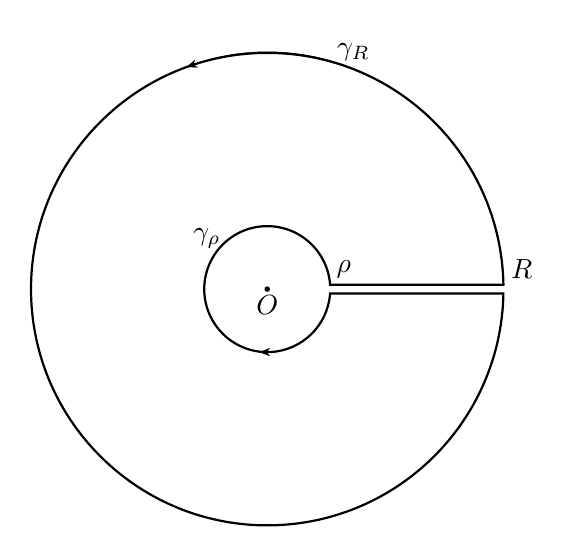
\begin{tikzpicture}[thick,every node/.style={inner sep=2pt},
		>={Stealth[width=3pt]}]
		\draw(4:0.8)node[above right]{$\rho$}--++(2.215,0)node[above right]{$R$}--++(-2.229,0)
		(3:0.8)arc(3:356:0.8)--++(2.215,0);
		\draw(1:3)arc(1:358.7:3);
		\draw[->,very thin](30:3)arc(30:110:3);
		\draw[->,very thin](0,-0.8)--++(-0.1,0);
		\draw(140:1)node{$\gamma_\rho$}(70:3.2)node{$\gamma_R$};
		\fill(0,0)circle(1pt)node[below]{$O$};
	\end{tikzpicture}
	\caption{\label{fig8.1}}
\end{figure}

\begin{theorem}[Green 定理]
	假设 $D \subset \mathbb{R}^2$ 是区域且 $P, Q$ 在 $D$ 上连续,则下列命题等价:

	\begin{itemize}
		\item 对 $D$ 内任意分段光滑曲线 $L$,曲线积分
		      \[ \int_L P \d x + Q \d y \]
		      与路径 $L$ 无关,只与 $L$ 的起点和终点有关。
		\item 如果存在 $U$ 使得 $\d U = P \d x + Q \d y$,即称 $P \d x + Q \d y$ 在 $D$ 上是正合的,称 $U$ 是其原函数。
		\item 沿着 $D$ 内任意分段光滑闭曲线 $L$,有
		      \[ \oint_{L} P \d x + Q \d y = 0 \]
	\end{itemize}
\end{theorem}

如果进一步假设 $P, Q$ 在 $D$ 上一阶导数连续,则在 $D$ 内处处成立
\[ \frac{\partial Q}{\partial x} = \frac{\partial P}{\partial y} \]
且和上面三条等价。

\subsection{Gauss 公式}

\begin{theorem}[Gauss 公式]
	设 $\Omega \subset \mathbb{R}^3$ 是区域且边界 $\partial \Omega$ 是由分段光滑的定向曲面构成。设 $P, Q, R$ 是一阶导数连续的,则
	\[ \iint_{\partial \Omega} P \d y \d z + Q \d z \d x + R \d x \d y = \iiint_{\Omega} \left( \frac{\partial P}{\partial x} + \frac{\partial Q}{\partial y} + \frac{\partial R}{\partial z} \right) \d x \d y \d z \]
\end{theorem}

\subsection{Stokes 公式}

\begin{theorem}[Stokes 公式]
	设 $\Sigma$ 是光滑定向曲面且边界 $\partial \Sigma$ 为分段光滑闭曲面,取诱导定向。对其上具有一阶连续偏导数的函数 $P, Q, R$ 有
	\[ \int_{\partial \Sigma} P \d x + Q \d y + R \d z = \iint_\Sigma \left| \begin{matrix}
			\d y \d z                   & \d z \d x                   & \d x \d y                   \\
			\frac{\partial}{\partial x} & \frac{\partial}{\partial y} & \frac{\partial}{\partial z} \\
			P                           & Q                           & R
		\end{matrix} \right| \]
\end{theorem}

\section{旋转体}

假设平面曲线 $y = f(x)$ 绕 $x$ 轴进行旋转,则旋转体体积为
\[ V = \pi \int_a^b f^2(x) \d x \]
假如曲线以 $y = \tan x$ 进行旋转,则
\[ V = \pi \int_a^b |x \cos \theta - y \sin \theta|^2(\cos \theta \d x + \sin \theta \d y) = \pi \int_a^b \frac{|yk-x|^2}{(k^2+1)^{\frac{3}{2}}}(y'k+1) \d x \]


    % 多变量理论
\chapter{概率论}

考研中遇到的概率论很少,暂放于此。

\section{随机事件与概率}

假定某个试验有有限个可能的结果 $e_1, \cdots, e_N$,其出现机会是等可能的。假定事件 $E$ 包含了其中的 $M$ 个结果,则称事件 $E$ 的概率为
\[ P(E) = M / N \]
这是古典概型。另一些时候,我们把结果扩展到无限的情况。我们把度量(可以通俗的理解为面积)相同的事件称为等可能的,这是几何概型。

称集合 $\Omega$ 随机事件的样本空间,其元素 $\omega$ 称为基本事件。事件 $A$ 是 $\Omega$ 的一个子集,赋给每个事件一个实数值 $P(A)$,称为概率。其满足要求:

\begin{itemize}
	\item 非负性:$P(A) \geqslant 0$。
	\item 规范性:$P(\Omega) = 1, P(\varnothing) = 0$。
	\item 加法公理。
\end{itemize}

若两个事件不能在同一次试验中同时发生,则称为互斥的。若一些事件中任意两个都互斥,则称为两两互斥。可以进一步导出对立事件的概念。可以把集合的交并补也引入。

\begin{theorem}[加法公理]
	若干个互斥事件之和的概率,等于各事件的概率之和:
	\[ P\left(\bigcup A_i\right) = \sum P(A_i) \]
\end{theorem}

\begin{note}
	这条公理其实是在古典定义、统计定义下是可证明的,但是为什么是公理呢?因为我们的确可以建立一种新的概率理论,在其中加法公理不成立。类似于平行公设。
\end{note}

\begin{definition}
	设 $A,B$ 是两个事件且 $P(A) > 0$,我们称在已知 $A$ 发生的条件下事件 $B$ 发生的概率为条件概率,记作
	\[ P(B | A) = \frac{P(AB)}{P(A)} \]
\end{definition}

假如 $P(B \mid A) > P(B)$,我们可以说事件 $A$ 促进了事件 $B$ 的发生。反之 $P(B \mid A) = P(A)$,则 $B$ 的发生对 $A$ 无影响。

形式的说:

\begin{definition}[条件概率]
	若两事件 $A, B$ 满足
	\[ P(A B) = P(A) P(B) \]
	则称 $A, B$ 独立。
\end{definition}

变换形式是为了避免 $0$ 的讨论。

设一列事件 $A_1, A_2, \cdots$,假如从中取出任意有限个都成立
\[ P(A_{i1} \cdots A_{im}) = P(A_{i1}) \cdots P(A_{im}) \]
那么称事件 $A_1, A_2, \cdots$ 相互独立。注意与两两独立的区别。


\begin{theorem}[全概率公式]
	设 $B_1, \cdots$ 为一列事件,他们两两互斥且每次试验至少发生一个。有时称这种性质为“完备事件群”。那么对任意事件 $A$ 有
	\[ P(A) = P(B_1)P(A \mid B_1) + P(B_2)P(A \mid B_2) + \cdots \]
\end{theorem}


\begin{theorem}[全概率公式]
	贝叶斯公式:对 $n$ 个两两不相容事件 $A_1, \cdots, A_n$,则对事件 $B$ 有
	\[ P\left(A_j | B\right) = \frac{P(A_j)P(B | A_j)}{\sum\limits_{i=1}^n P(A_i)P(B | A_i) } \]
\end{theorem}

\begin{note}
	若 $P(AB) = 0$,不意味着 $AB = \varnothing$。比如 $[0,1]\cap [1,2] = \{1\}$,但概率是 $0$。
\end{note}

\section{一维随机变量及其分布}

随机变量就是“其值会随机而定”的变量,是一个实值单值函数。设随机实验的样本空间为 $\Omega$,若对于任意 $\omega \in \Omega$ 都有唯一实数 $X(\omega)$ 与其对应,且对任意实数 $x$,$\{\omega \mid X(\omega) \leqslant x, \omega \in \Omega\}$ 是随机时间,则称定义在 $\Omega$ 上的实值单值函数为随机变量。

\paragraph{离散型随机变量}

研究一个随机变量,不只是查看其能取哪些值,更要看其取各种值的概率如何。

\begin{definition}
	设 $X$ 是离散型随机变量,其全部可能值为 $\{a_1, \cdots\}$,则称
	\[ p_i = P\{X = a_i\} \]
	为其概率函数。称
	\[ F(x) = P\{X \leqslant x\} = \sum_{a_i \leqslant x} p_i \]
	是其分布函数。记为 $X \sim F(x)$,称 $X$ 服从 $F(x)$ 分布。
\end{definition}

其具有以下的性质:

\begin{itemize}
	\item $F(x)$ 对 $x$ 单调不减。
	\item $F(x)$ 是 $x$ 的右连续函数。
	\item $F(- \infty) = \lim\limits_{i \to -\infty} F(x) = 0$,$F(+\infty) = \lim\limits_{x \to + \infty} F(x) = 1$。
	\item $P\{X \leqslant a\} = F(a)$,$P\{X < a\} = F(a - 0)$,$P\{X = a\} = F(a) - F(a - 0)$。
\end{itemize}

如果随机变量只取有限的可列值,则称为离散型随机变量,可以写分布列。

\paragraph{连续型随机变量}

如果随机变量的分布函数是 $F(x)$,则 $f(x) = F'(x)$ 是其的概率密度函数。

其具有以下的性质:

\begin{itemize}
	\item $f(x) \geqslant 1$。
	\item 对任何常数 $a, b$ 有
	      \[ P\{a \leqslant X \leqslant b\} = F(b) - F(a) = \int_{a}^{b} f(x) \d x, \qquad \int_{-\infty}^{\infty} f(x) \d x = 1 \]
\end{itemize}

\subsection{常见随机分布}

\paragraph{二项分布}
如果 $X$ 的概率分布为
\[ P\{X = k\} = \binom{n}{k} p^k(1 - p)^{n-k}. \quad k = 0, 1, \cdots, n \]
则称 $X$ 服从参数为 $(n, p)$ 的二项分布,记为 $X \sim B(n, p)$。特别的,当 $n=1$ 时称为二项分布。二项分布也是 $n$ 重伯努利实验中事件 $A$ 发生的次数,其中 $P(A) = p$。

\paragraph{泊松分布}
如果 $X$ 的概率分布为
\[ P\{X = k\} = \frac{\lambda^k}{k!} \ee^{-\lambda} , \quad k = 0, 1, \cdots \]
则记为 $X \sim P(\lambda)$。

\paragraph{几何分布}
如果 $X$ 的概率分布为
\[ P\{X=k\} = (1 - p)^{k-1}p, \quad k = 1, 2, \cdots \]
则记为 $X \sim G(p)$。

\paragraph{超几何分布}
如果 $X$ 的概率分布为
\[ P\{X = k\} = \frac{\binom{M}{k} \binom{N - M}{n - k}}{\binom{N}{n}}, \quad \max(0, n - N + M) \leqslant k \leqslant \min(M, n) \]
则记为 $X \sim H(n, N, M)$。设有 $N$ 个产品组成的整体,其中有 $M$ 个不合格产品,从中取出 $n$ 个,次品数为 $k$,这就是组合意义。

\paragraph{均匀分布}
如果 $X$ 的概率密度函数为
\[ f(x) = \frac{1}{b - a}, \quad a < x < b \]
则记为 $X \sim U(a, b)$。

\paragraph{指数分布}
如果 $X$ 的概率密度函数为
\[ f(x) = \lambda \ee^{-\lambda x}, \quad x > 0 \]
则记为 $X \sim E(\lambda)$。

\paragraph{正态分布}
如果 $X$ 的概率密度为
\[ f(x) = \frac{1}{\sqrt{2 \pi}  \sigma} \exp \left(- \frac{(x - \mu)^2}{2\sigma^2}  \right) \]
则记为 $X \sim N(\mu, \sigma^2)$。

\section{多维随机变量}

设 $X = (X_1, \cdots, X_N)$,其中每个分量都是一维随机变量,则 $X$ 是一个 $n$ 维随机变量。

\paragraph{离散型}

假如每个分量是离散型的,那么称 $X$ 是 $n$ 维离散型随机变量。

\begin{definition}
	以 $\{a_{i1}, \cdots\}$ 记 $X_i$ 的全部可能值,则事件的概率
	\[ p(j_1, \cdots, j_n) = P\{X_1 = a_{1j_1}, \cdots, X_n = a_{n j_n}\} \]
	为随机变量的概率函数。显然应该满足条件
	\[ p(j_1, \cdots) \geqslant 0, \quad \sum_{j_n} \cdots \sum_{j_1} p(j_1, \cdots)  =1 \]
\end{definition}

\paragraph{连续型}
连续型随机变量不能简单的定义为各分量都是“一维连续型随机变量的那种”。考虑 $X_1 = X_2$,则 $(X_1, X_2)$ 仅在对角线处有值,故不可能存在概率密度函数。

\begin{definition}
	设 $f(x_1, \cdots, x_n)$ 是定义在 $\mathbb{R}^n$ 上的非负函数,使得对 $\mathbb{R}^n$ 中的任何集合 $A$,有
	\[ P\{X \in A\} = \int_A \cdots \int f(x_1, \cdots, x_n) \d x_1 \cdots \d x_n \]
	则称 $f$ 是 $X$ 的概率密度函数。显然当 $P\{ X \in \mathbb{R}^n\} = 1$。
\end{definition}

也可以定义分布函数
\[ F(x_1, \cdots, x_n) = P\{X_1 \leqslant x_1, \cdots, X_n \leqslant x_n \} \]

对于二维 $(X, Y)$,若 $f$ 在点 $(x, y)$ 处连续,则
\[ \frac{\partial^2 F(x, y)}{\partial x \partial y} = f(x, y) \]
反之若 $F(x, y)$ 连续可导,则此式是其概率密度。

\paragraph{边缘分布}

对任意的 $n$ 个实数,$x_1, x_2, \cdots, x_n$,称 $n$ 元函数
\[ F(x_1, \cdots, x_n) = P\{X_1 \leqslant x_1, X_2 \leqslant x_2, \cdots. X_n \leqslant x_n\} \]
为多维随机变量 $(X_1, \cdots, X_n)$ 的联合分布函数,记为 $(X_1, \cdots, X_n) \sim F(x_1, \cdots, x_n)$。

\begin{itemize}
	\item $F(x, y)$ 是 $x, y$ 的单调不减函数。
	\item $F(x, y)$ 是 $x, y$ 的右连续函数。
	\item $F(-\infty, y) = F(x, -\infty) = F(-\infty, -\infty) = 0$,$F(+\infty, +\infty) = 1$。
	\item 对任意 $x_1 < x_2, y_1 < y_2$,有
	      \[ P\{x_1 < X \leqslant x_2, y_1 Y \leqslant y_2\} = F(x_2, y_2) - F(x_2, y_1) - F(x_1, y_2) + F(x_1, y_1) \geqslant 0 \]
\end{itemize}

设其联合分布函数为 $F(x,y)$,定义边缘分布函数
\[ F_X(x) = P\{X \leqslant x\} = F(x, +\infty) \]
同理,有 $F_Y(y) = F(+\infty, y)$。


\subsection{常见的二维分布}

\paragraph{二维均匀分布} 称 $(X,Y)$ 在平面有界区域 $D$ 上服从均匀分布,如果 $(X, Y)$ 的概率密度为
\[ f(x, y) = \frac{1}{S_D}, \quad (x, y) \in D \]

\paragraph{二维正态分布} TODO。

\subsection{二维随机变量的独立性}

\paragraph{条件概率分布}

对于二维离散型随机向量 $(X, Y)$,其联合概率分布为
\[ p_{i,j} = P\{X= x_i, Y = y_j\} \]
记为 $(X,Y) \sim p_{i,j}$。依条件概率的定义,有
\[ P\{ X = x_i \mid Y = y_i \} = \frac{P\{X = x_i, Y = y_j\}}{P\{Y=y_j\}} = \frac{p_{i, j}}{p_{, j}} \]

设二维连续型随机向量 $(X, Y)$,其概率密度是 $f(x, y)$。假设 $y \in [a, b]$,依条件概率的定义,有
\[ P\{X \leqslant c \mid a \leqslant Y \leqslant b\} = \frac{P\{X \leqslant c , a \leqslant Y \leqslant b\}}{P\{a \leqslant y \leqslant b \}} = \frac{\int_{-\infty}^c \int_{a}^b f(x, y) \d y \d x }{\int_a^b f_Y(y) \d y }\]
对 $c$ 求导,即得条件密度函数
\[ f_{X \mid Y}(x \mid a \leqslant y \leqslant b) = \frac{\int_{a}^b f(x, y) \d y}{\int_{a}^b f_{Y}(y) \d t} \]
考虑极限,$a, b$ 收敛于 $y$ 处,有
\[ f_{X \mid Y}(x \mid y) = \frac{f(x, y)}{f_{Y}(y)} \]

\paragraph{独立性}

与一维情况类似,我们可以推广为 $n$ 维。

\begin{definition}
	设 $n$ 维随机向量 $(X_1, \cdots, X_n)$ 的联合密度函数为 $f(x_1, \cdots, x_n)$,而 $f_i$ 是 $X_i$ 的边缘密度函数,若
	\[ f(x_1, \cdots, x_n) = f_1(x_1) \cdots f_n(x_n) \]
	则称随机变量 $X_1, \cdots, X_n$ 相互独立。
\end{definition}

\paragraph{随机变量函数的概率分布}

离散的情况是容易的,实在不行手算。

设连续型随机变量 $X$ 有密度函数 $f(x)$,对于函数 $g$,考虑 $Y=g(X)$ 下的情况。假设 $g$ 严格上升,设 $h = g^{-1}$,有
\[ P\{Y \leqslant y\} = P\{X \leqslant h(y)\} = \int_{-\infty}^{h(y)} f(t) \d t \]
则 $y$ 的密度函数为
\[ l(y) = f(h(y)) h'(y) \]
同理,对严格递减也可以进行讨论,得到结论
\[ l(y) = f(h(y)) |h'(y)| \]

例如 $Y = aX+b$,则 $Y$ 的密度函数为
\[ l(y) = \frac{1}{|a|}f\left(\frac{y-b}{a}\right) \]

现考虑二元情况 $(X_1, X_2)$ 的密度函数为 $f(x_1, x_2)$,并有变量
\[ Y_1 = g_1(X_1, X_2), \quad Y_2 = g_2(X_1, X_2) \]
假定存在逆变换
\[ X_1 = h_1(Y_1, Y_2), \quad X_2 = h_2(Y_1, Y_2) \]
此时 Jacobi 行列式
\[ J(y_1, y_2) = \left|\begin{matrix}
		\partial h_1 / \partial y_1 & \partial h_1 / \partial y_2 \\
		\partial h_2 / \partial y_1 & \partial h_2 / \partial y_2
	\end{matrix}\right| \]
不为 $0$。在 $(Y_1, Y_2)$ 的平面上任取一个区域 $A$,对应于 $(X_1, X_2)$ 上的区域是 $B$。即
\[ \begin{aligned}
		P\{(Y_1, Y_2) \in A\} & = P\{(X_1, X_2) \in B\}                                                      \\
		                      & = \iint_{B} f(x_1, x_2) \d x_1 \d x_2                                        \\
		                      & = \iint_{A} f(h_1(y_1, y_2), h_2(y_1, y_2)) \cdot |J(y_1, y_2) \d y_1 \d y_2
	\end{aligned} \]
因此 $(Y_1, Y_2)$ 的概率密度为
\[ l(y_1, y_2) = f(h_1(y_1, y_2), h_2(y_1, y_2)) | J(y_1, y_2)| \]

比较常见的例子是线性变换
\[ Y_1 = a_{11} X_1 + a_{12} X_2, \quad Y_2 = a_{21} X_1 + a_{22} X_2 \]
当其行列式不为 $0$ 时,设其存在逆变换
\[ X_1 = b_{11} Y_1 + b_{12} Y_2, \quad X_2 = b_{21} Y_1 + b_{22} Y_2 \]
可得
\[ l(y_1, y_2) = f(b_{11} y_1 + b_{12} y_2, b_{21} y_1 + b_{22} y_2) | b_{11} b_{22} - b_{12} b_{21} | \]

\section{随机变量的数字特征}

设 $X$ 是随机变量,其分布列为 $p_i = P\{X = x_i\}$,记
\[ E(X) = \sum_{i=1}^\infty x_i p_i \]
为随机变量 $X$ 的数学期望。若 $X$ 是连续型随机变量,则记
\[ E(X) = \int_{-\infty}^{+\infty} x f(x) \d x \]
为其期望。

其拥有线性性。比如设 $X, Y$ 相互独立,有
\[ E(X Y) = E(X) E(y), \quad E(X \pm Y) = E(X) \pm E(Y) \]

我们记 $E[(X - E(X))^2]$ 为 $X$ 的方差,有
\[ D(X) = E[(X - E(X))^2] = E(X^2) - (E(X))^2 \]
称 $\sqrt{D(X)}$ 为 $X$ 的标准差,或者均方差,记为 $\sigma(X)$。

\begin{theorem}[切比雪夫不等式]
	如果随机变量 $X$ 的期望 $E(X)$ 和方差 $D(X)$ 存在,则对任意 $\eps > 0$ 有
	\[ P\{|X - E(X)| < \eps\} \geqslant 1 - \frac{D(X)}{\eps^2} \]
\end{theorem}

我们定义 $(X, Y)$ 的协方差为
\[ \Cov(X, Y) = E[(X - E(X)(Y - E(Y)))] = E(XY) - E(X) E(Y) \]

称 $\rho_{XY} = \frac{\Cov(X, Y)}{\sqrt{D(X) D(Y)}}$ 为 $X, Y$ 的相关系数。

\section{大数定律与中心极限定理}

设随机变量 $X$ 与随机变量序列 $\{X_n\}$,如果对任意的 $\eps > 0$ 有
\[ \lim_{n \to \infty} P\{|X_n - X| < \eps \} =1 \]
则称随机变量序列 $\{X_n\}$ 依概率收敛于随机变量 $X$,记为
\[ \lim_{n \to \infty} X_n = X(P), \quad \text{或}\ X_n \stackrel{P}{\longrightarrow} X(n \to \infty) \]

\begin{theorem}[切比雪夫大数定律]
	设 $\{X_n\}$ 是相互独立的随机变量序列,如果方差 $D(X)$ 存在且有一致有上界,则 $\{X_n\}$ 服从大数定律
	\[ \frac{1}{n} \sum_{i=1}^n X_i \stackrel{P}{\longrightarrow} \frac{1}{n} \sum_{i=1}^n E(X_i) \]
\end{theorem}

\begin{theorem}[伯努利大数定律]
	假设 $\mu_n$ 是 $n$ 重伯努利实验中时间 $A$ 发生的次数,在每次实验中 $A$ 发生的概率为 $p(0 < p < 1)$,则
	\[ \frac{\mu_n}{n} \stackrel{P}{\longrightarrow} p \]
\end{theorem}

\begin{theorem}[辛钦大数定律]
	设 $\{X_n\}$ 是独立同分布的随机变量序列,如果 $E(X_i) = \mu$ 存在,则
	\[ \frac{1}{n} \sum_{i=1}^n X_i \stackrel{P}{\longrightarrow} \mu \]
\end{theorem}

\begin{theorem}[列维 - 林德伯格定理]
	假设 $\{X_n\}$ 是独立同分布的随机变量序列,如果
	\[ E(X_i) = \mu, D(X_i) = \sigma^2 > 0 \]
	存在,则对任意的实数 $x$ 有
	\[ \lim_{n \to \infty} P\left\{ \frac{\sum_{i=1}^n X_i - n \mu}{\sigma \sqrt{n}} \leqslant x \right\} = \frac{1}{\sqrt{2 \pi}} \int_{-\infty}^x \exp\left(-\frac{t^2}{2}\right) \d t = \Phi(x)  \]
\end{theorem}

\begin{theorem}[棣莫弗 - 拉普拉斯定理]
	设随机变量 $Y_n \sim B(n, p)$,其中 $0 < p < 1$ 且 $n > 1$,则对任意的实数 $x$,有
	\[ \lim_{n \to \infty} P\left\{ \frac{Y_n - np}{\sqrt{np(1 - p)}} \leqslant x \right\} = \frac{1}{\sqrt{2 \pi}} \int_{-\infty}^x \exp\left(-\frac{t^2}{2}\right) \d t = \Phi(x)  \]
\end{theorem}

\section{数理统计}

研究对象的全体称为总体,组成总体的每一个元素称为个体。我们把总体和 $X$ 等同起来,所谓总体的分布就是指 $X$ 的分布。

$n$ 个相互独立且与总体 $X$ 具有相同概率分布的随机变量 $X_1, \cdots, X_n$ 所组成的总体为 $(X_1, \cdots, X_n)$ 称为来自总体 $X$ 容量为 $n$ 的一个简单随机样本,简称样本。一次抽样结果的 $n$ 个具体数值称为 $X_1, \cdots, X_n$ 的一个观测值(样本值)。

假设总体 $X$ 的分布函数为 $F$,则 $(X_1, \cdots, X_n)$ 的分布函数为
\[ F(x_1, \cdots, x_n) = \prod_{i=1}^n F(x_i) \]

设 $X_1, \cdots, X_n$ 为来自总体 $X$ 的一个样本,$g$ 为仅与 $x$ 有关的 $n$ 元函数,则称 $g$ 为样本的一个统计量。若 $(x_1, \cdots, x_n)$ 为样本值,则 $g(x_1, \cdots, x_n)$ 为观测值。

样本均值
\[ \overline{X} = \frac{1}{n} \sum_{i=1}^n X_i \]
样本方差
\[ S^2 = \frac{1}{n-1} \sum_{i=1}^n (X_i - \overline{X})^2 \]
样本 $k$ 阶(原点)矩
\[ A_k = \frac{1}{n} \sum_{i=1}^n X_i^k \]
样本 $k$ 阶中心矩
\[ B_k = \frac{1}{n} \sum_{i=1}^n (X_i - \overline{X})^k \]

将 $n$ 个观测量从小到大的顺序排列,记随机变量 $X_{(k)}$ 为第 $k$ 顺序统计量。

常用统计量:

\[
	\begin{aligned}
		E(X_i)          & = E(X)             \\
		D(X_i)          & = D(X)             \\
		E(\overline{X}) & = E(X)             \\
		D(\overline{X}) & = \frac{1}{n} D(X) \\
		E(S^2)          & = D(X)
	\end{aligned}
\]

\subsection{三大分布}

\newcommand{\calX}{\mathcal{X}}

\paragraph{$\calX^2$ 分布}

若随机变量 $X_1, \cdots, X_n$ 相互独立且都服从标准正态分布,则随机变量 $X = \sum X_i^2$ 服从自由度为 $n$ 的 $\calX^2$ 分布,记为 $X \sim \calX^2(n)$。

对于给定的 $\alpha(0 < \alpha < 1)$,称满足
\[ P\left\{\calX^2 > \calX_\alpha^2(n)\right\} = \int_{\calX_\alpha^2(n)}^n f(x) \d x = \alpha  \]
的 $\calX_\alpha^2(n)$ 为 $\calX^2(n)$ 分布的上 $\alpha$ 分位点。

\paragraph{$t$ 分布}

设随机变量 $X \sim N(0, 1), Y \sim \calX^2(n)$,$X$ 与 $Y$ 互相独立,则随机变量 $t = \frac{X}{\sqrt{Y / n}}$ 服从自由度为 $n$ 的 $t$ 分布,记为 $t \sim t(n)$.

\paragraph{$F$ 分布}

设随机变量 $X \sim \calX^2(n_1), y \sim \calX^2(n_2)$,且 $X$ 与 $Y$ 相互独立,则 $F = \frac{X / n_1}{Y / n_2}$ 服从自由度为 $(n_1, n_2)$ 的 $F$ 分布,记为 $F \sim F(n_1, n_2)$。

\subsection{参数的点估计}

设总体 $X$ 的分布函数为 $F(x; \theta)$,其中 $\theta$ 是一个未知参数,$X_1, \cdots, X_n$ 是取自总体 $X$ 的一个样本。由样本构造一个适当的统计量 $\hat{\theta}(X_1, \cdots, X_n)$ 作为参数 $\theta$ 的估计,则称 $\hat{\theta}$ 为其估计量。

如果 $x_1, \cdots, x_n$ 是样本的一个观察值,将其带入估计量得值 $\hat{\theta}(x_1, \cdots, x_n)$ 并以此值作为未知参数的近似值,则称为 $\theta$ 的估计值。

\paragraph{矩估计法}

设总体 $X$ 分布有 $n$ 个样本,有 $k$ 个未知参数。若 $X$ 的原点矩存在,我们令样本矩等于总体矩
\[ \frac{1}{n} \sum_{i=1}^{N} X_i^l = E(X^l), \quad l = 1, \cdots, k \]
这是包含 $k$ 个参数的 $k$ 个方程,由此解得矩估计量和矩估计值。

一般约定:用矩法方程求总体未知参数的估计量时,从低阶开始。

\paragraph{最大似然估计法}

最大似然原理:对未知参数 $\theta$ 进行估计时,在该参数可能的取值范围 $I$ 内选取,用使”样本获得观测值 $x_1, \cdots, x_n$ 的概率最大的参数值 $\hat{\theta}$ 作为 $\theta$ 的估计。

假设 $X$ 是离散型随机变量,其概率分布为 $P\{X = x\} = p(x; \theta)$,那么求其取值概率
\[ L(x_1, \cdots, x_n;\theta) = P\{X_1 = x_1, \cdots, X_n = x_n\} = \prod_{i=1}^n P\{X_i=x_i\} = \prod_{i=1}^n p(x_i; \theta) \]
称为样本的似然函数。若存在 $\hat{theta}$ 使得 $L$ 取到最大值,则称 $\hat{theta}$ 为最大似然估计值,对应的统计量是 $\theta$ 的最大似然估计量。

同理,连续型随机变量也有
\[ L(x_1, \cdots, x_n; \theta) = \prod_{i=1}^n f(x_i; \theta) \]



    % 概率论

\chapter{习题}

\section{函数、极限、连续}

\begin{problem}[000001]
设 $a_1=1,a_k=k(a_{k-1}+1)$,试计算
\[ \lim_{n\to \infty}\prod_{k=1}^n\left(1+\frac{1}{a_k}\right)\]
\end{problem}
\begin{solution}
	先变形
	\[ \left(1+\frac{1}{a_k}\right)=\frac{a_{n+1}}{ka_n}\]
	累乘可以化简
	\[ \prod_{k=1}^n\left(1+\frac{1}{a_k}\right) = \frac{a_{n+1}}{(n+1)!}\]
	注意到
	\[ \frac{a_{n+1}}{(n+1)!}-\frac{a_{n}}{n!} = \frac{a_{n+1}-(n+1)a_n}{(n+1)!} = \frac{1}{n!}\]
	故
	\[ \lim_{n\to \infty}\prod_{k=1}^n\left(1+\frac{1}{a_k}\right) = \lim_{n\to \infty}\left(1+\frac{1}{2!}+\cdots+\frac{1}{n!}\right) = \ee\]
\end{solution}

\begin{problem}[000002]
设 $x_1 = 2, x_n + (x_n - 4)x_{n-1} = 3(n = 2, 3, \cdots)$,求 $\displaystyle\lim_{n\to \infty} x_n$。
\end{problem}

\begin{solution}
	显然是考不动点。

	考虑方程
	\[ x + (x-4)x - 3 = x^2 - 3x - 3 = 0 \]
	的解,取其中一解 $x_0 = \frac{3 + \sqrt{21}}{2}$。接下来考察单调性,设 $x_{n-1} \in [2, x_0)$,有
	\[ x_n - x_{n-1} = 4 - x_{n-1} - \frac{1}{x_n - 1} = -\frac{x_{n-1}^2 - 3x_{n-1} - 3}{x_{n-1} - 1} > 0 \]
	故序列 $\{x_n\}$ 单调递增且 $x_n \in [2, x_0)$。设极限为 $A$,解方程
	\[ A^2 - 3A - 3 = 0, \quad A = x_0 = \frac{3 + \sqrt{21}}{2} \]
\end{solution}

\begin{problem}[000003]
是否存在这样的函数,它在区间 $[0,1]$ 上每点取有限值,在此区间的任何点的任一邻域内无界。
\end{problem}
\begin{solution}
	构造
	\[ f(x) = \begin{cases}
			n, & x=\dfrac{m}{n},m,n\ \text{为互质整数} \\
			0, & x\ \text{为无理数}
		\end{cases} \]
\end{solution}

\begin{problem}[000004]
设 $f,g$ 是 $\mathbb{R}$ 上的实函数,且
\[ f(x+y)+f(x-y) = 2f(x)g(y)\]
在 $\mathbb{R}$ 上 $f(x)$ 不恒等于零但有界,试证:$|g(y)|\leqslant 1$
\end{problem}
\begin{solution}
	令 $M=\sup|f(x)|$,则有
	\[ 2M\geqslant |f(x+y)|+|f(x-y)| \geqslant |f(x+y)+f(x-y)| = 2|f(x)||g(y)| \]
	设存在 $y_0$ 使得 $|g(y_0)|=1+2\delta>1$。由上确界的定义知存在 $x_0$ 有
	\[ M \geqslant |f(x_0)| > \frac{M}{\delta+1}\]
	故
	\[ 2|f(x_0)||g(y_0)| > \frac{2(1+2\delta)M}{1+\delta} > 2M\]
	因此矛盾,故恒有 $|g(y)|\leqslant 1$。
\end{solution}


\begin{problem}[000005]
设 $f$ 是闭区间 $[a,b]$ 上的增函数(但不一定连续),如果 $f(a) \geqslant a,f(b) \leqslant b$,试证: $\exists x_0 \in [a,b]$,使得 $f(x_0) = x_0$。
\end{problem}
\begin{solution}
	设 $A=\{x \mid f(x) \geqslant x\}$,由题知 $a\in A$ 故 $A$ 非空。又 $f$ 定义在 $[a,b]$ 上,故 $A$ 有界。因此设 $x_0=\sup A\in [a,b]$ 是有意义的。又 $f(x)\in[a,b]$ 在定义域内,分类讨论如下

	1. 若 $y_0=f(x_0) > x_0$,由单调性知
	\[ f(y_0)=f(f(x_0)) \geqslant f(x_0) = y_0\]
	故 $y_0\in A$。这意味着 $\sup A \geqslant y_0 >x_0$,矛盾。

	2. 若 $y_0=f(x_0) < x_0$,由确界定义知 $\exists x_1\in A$ 使 $y_0<x_1\leqslant x_0$,由单调性知
	\[ f(x_1)\leqslant f(x_0)=y_0 <x_1\]
	这意味着 $x_1\notin A$,矛盾。

	故 $y_0=f(x_0)=x_0$,此时 $x_0 = \sup\{x \mid f(x) \geqslant x\}$。

	注意 $x_0$ 不一定在 $A$ 中,即 $f(x_0) \geqslant x_0$ 不一定成立。
\end{solution}


\begin{problem}[000006]
设 $f(x)$ 是定义在 $\mathbb{R}$ 上的函数且对任意 $x,y$有
\[ |xf(y)-yf(x)| \leqslant M|x|+M|y|\]
其中 $M > 0$。求证:存在常数 $a$ 使得对任意 $x$ 有 $|f(x)-ax| \leqslant M$
\end{problem}
\begin{solution}
	当 $x=0$ 时,有 $|f(0)|\leqslant M$。而当 $xy\ne 0$ 时,恒有
	\[ \left| f(x)-\frac{f(y)}{|y|}x \right| \leqslant M \left(1+\frac{|x|}{|y|}\right)\]
	若 $a$ 不存在,即对任意的 $a$ 存在 $x_0$ 使
	\[ |f(x_0)-ax_0|=M(1+2\delta)>M\]
	那么取 $a = \dfrac{f(y_0)}{|y_0|}$,当 $y_0=\dfrac{|x_0|}{\delta}$ 时,有
	\[ \left| f(x)-\frac{f(y_0)}{|y_0|}x \right| \leqslant M \left(1+ \frac{|x_0|}{|y_0|}\right)=M(1+\delta)\]
	因此矛盾,故存在 $a$。
\end{solution}

\begin{problem}[000007]
设 $\displaystyle\lim_{n\to\infty}a_n=A$,求证:$\displaystyle\lim_{n\to\infty}\frac{\sum a_n}{n}=A$。
\end{problem}

\begin{solution}
	即对于任给的 $\eps>0$,存在 $n>N_1$ 使得
	\[ |a_n-A|<\dfrac{\eps}{2}\]
	那么变形有
	\[ \left|\frac{\sum a_n}{n}-A\right| \leqslant \frac{\sum |a_n-A|}{n} = \frac{\sum_{k=1}^{N_1} |a_k-A|}{n} + \frac{\sum_{k=N_1+1}^{n} |a_k-A|}{n}\]
	注意到 $\sum_{k=1}^{N_1} |a_k-A|$ 已经为定值,从而存在 $n>N_2$ 使得
	\[ \frac{\sum_{k=1}^{N_1}|x_k-A|}{n}<\frac{\eps}{2}\]
	因此当 $n>\max\{N_1,N_2\}$ 时有
	\[ LHS < \frac{\eps}{2}+\frac{n-N_1}{n}\times \frac{\eps}{2} < \frac{\eps}{2}+\frac{\eps}{2} = \eps \]
\end{solution}

\begin{problem}[000017]
已知 $\lim\limits_{x \to +\infty} f(x)$ 存在,且
\[ f(x) = \frac{x^{1+x}}{(1+x)^x} - \frac{x}{\ee} + 2 \lim_{x \to \infty} f(x) \]
求 $f(x)$。
\end{problem}

\begin{solution}
	显然先取 $t = \frac{1}{x}$,设极限为 $A$,则
	\[ A = 2A + \lim_{t \to 0^+} \left( \frac{1}{t (t+1)^{\frac{1}{t}}} - \frac{1}{t \ee} \right) \]
	故取等价无穷小得
	\[ -A = \lim_{t \to 0^+} \frac{1 - \exp\left( \frac{\ln(t + 1)}{t} - 1\right)}{t \exp\frac{\ln(t + 1)}{t}} = \lim_{t \to 0^+} \frac{1 - \frac{\ln(t + 1)}{t}}{t \ee} = \frac{1}{2 \ee} \]
	因此
	\[ f(x) = \frac{x^{1+x}}{(1+x)^x} - \frac{x + 1}{\ee} \]
\end{solution}

\begin{problem}[000019]
设数列 $\{x_n\}$ 满足 $0 < x_n < \frac{\pi}{2}$,且
\[ \cos x_{n+1} - x_{n+1} = \cos x_n \]

(1) 计算 $\lim\limits_{n \to \infty} x_n$。

(2) 计算 $\lim\limits_{n \to \infty} \frac{x_{n+1}}{x_n^2}$。

\end{problem}

\begin{solution}
	(1) 因为
	\[ \cos x_{n+1} - \cos x_n = x_{n+1} > 0 \]
	且 $0 < x_n < \frac{\pi}{2}$,因此 $0 < x_{n+1} < x_n$。故极限存在。

	设极限为 $a$,由 $\cos a - a = \cos a$,易得 $a = 0$。

	(2) 由于 $\cos x \sim 1 - \frac{x^2}{2}$,故
	\[ \lim_{n \to \infty} \frac{x_{n+1}}{x_n^2} = \lim_{n \to \infty} \frac{x_{n+1}}{2 - 2 \cos x_{n}} = \lim_{n \to \infty} \frac{x_{n+1}}{2 - 2 \cos x_{n+1} + 2x_{n+1}} = \frac{1}{2} \]
\end{solution}

\begin{problem}[000030]
设
\[ x_{n+1} = 2 + \frac{1}{x_n}, \quad x_1 = 2 \]
求 $\lim\limits_{n \to \infty} x_n$。
\end{problem}

\begin{solution}
	设 $A = 2 + \frac{1}{A}$,取正解 $A = 1 + \sqrt{2}$。容易由数学归纳法证得 $x_n \in [2, \frac{5}{2}]$,注意到
	\[ |x_{n+1} - A| = \left|2 + \frac{1}{x_n} - A\right| = \frac{1}{Ax_n} |x_n - A| \leqslant \frac{1}{2A} |x_n - A| \]
	因此 $\lim\limits_{n \to \infty} x_n = A = 1 + \sqrt{2}$。

	也可以奇偶分开讨论单调性。
\end{solution}

\begin{problem}[000031]
设 $f(x)$ 在 $[0, 1]$ 上连续,且 $f(0) = f(1)$。证明:对于任意的 $n \in \mathbb{N}$,在 $[0, 1]$ 上至少存在一个 $\xi$ 使得
\[ f\left(\xi + \frac{1}{n}\right) = f(\xi) \]
\end{problem}

\begin{solution}
	设 $F(x) = f(x + \frac{1}{n}) - f(x)$,即证其在 $[0, 1 - \frac{1}{n}]$ 上有零点。注意到取一些点
	\[ \sum_{i=0}^{n - 1} F \left(\frac{i}{n}\right) = f(1) - f(0) = 0 \]
	则要么 $F$ 在这些点上值都为零,否则至少存在两个值异号,由介值定理知也存在零点。
\end{solution}

\section{一元微分学}

\begin{problem}[000009]
设 $f(z)$ 在 $[0,1]$ 上具有一阶连续导数,$f(0) = 0$,证明:存在$\xi \in [0,1]$,使得
\[ f'(\xi) = 2\int_0^1f(x) \d x \]
\end{problem}

\begin{solution}
	TODO。设上下界 $m, M$,中值定理。
\end{solution}

\begin{problem}[000010]
设 $f(x)$ 在 $[0, 1]$ 上连续,在 $(0, 1)$ 内可导,且 $f(0) = 0, f(1) = 1$,证明存在不同的 $\xi_1, \xi_2 \in (0, 1)$,使得
\[ \frac{1}{f'(\xi_1)} + \frac{1}{f'(\xi_2)} = 2 \]
\end{problem}

\begin{solution}
	由于连续,即存在 $x_0 \in (0, 1)$ 使得 $f(x_0) = \frac{1}{2}$。由中值定理,存在 $\xi_1 \in (0, x_0)$ 使得
	\[ f'(\xi_1) = \frac{f(x_0) - f(0)}{x_0 - 0} = \frac{1}{2x_0}
	\]
	同理,存在 $\xi_2 \in (x_0, 1)$ 使得
	\[ f'(\xi_2) = \frac{f(1) - f(x_0)}{1 - x_0} = \frac{1}{2(1 -x_0)} \]
	故
	\[ \frac{1}{f'(\xi_1)} + \frac{1}{f'(\xi_2)} = 2x_0 + 2(1 - x_0) = 2 \]

\end{solution}

\begin{problem}[000011]
设 $f(x)$ 在 $[0, 3]$ 上连续,在 $(0, 3)$ 内可导,且 $f(0) + f(1) + f(2) = 3, f(3) = 1$,证明存在 $\xi \in (0, 3)$,使得 $f'(\xi) = 0$。
\end{problem}

\begin{solution}
	TODO。设 $f(c) = f(3) = 1, c \in (0, 2)$。套中值定理。
\end{solution}

\begin{problem}[000012]
设 $f(x)$ 在 $[0, 1]$ 上连续,在 $(0, 1)$ 内可导,且
\[ f(1) = k \int_{0}^{\frac{1}{k}} x \ee^{1-x} f(x) \d x (k > 1) \]
证明至少存在一点 $\xi \in (0, 1)$,使得 $f'(\xi) = (1 - \xi^{-1})f(\xi)$。
\end{problem}

\begin{solution}
	TODO。构造 $F(x) = x \ee^{1-x} f(x)$。套中值定理。
\end{solution}

\begin{problem}[000013]
设 $f(x)$ 在 $[0, 1]$ 上连续,在 $(0, 1)$ 内二阶可导,过点 $A(0, f(0))$ 与 $B(1, f(1))$ 的直线与曲线 $y=f(x)$ 相交于点 $C(c, f(c))$,其中 $0 < c < 1$,证明存在 $\xi \in (0, 1)$,使得 $f''(\xi) = 0$。
\end{problem}

\begin{solution}
	TODO。构造 $F(x) = (1-x)f(0) + xf(1) - f(x)$,有 $F(0) = F(1) = F(c) = 0$。套中值定理。
\end{solution}

\begin{problem}[000016]
设 $f(x)$ 在 $[a, b]$ 上连续,在 $(a, b)$ 上导函数连续,且存在 $c \in (a, b)$ 使得 $f'(c) = 0$。证明:存在 $\xi \in (a, b)$,使得
\[ f'(\xi) - f(\xi) + f(a) = 0 \]
\end{problem}

\begin{solution}
	几何角度很直观,即 $\frac{f'(x) - f(a)}{f'(x)}$ 存在值为 $1$ 的时候。但是零点很恼人,严谨的说明是要费一番功夫的。

	积分构造
	\[ F(x) = \frac{f(x) - f(a)}{\ee^x}, \quad F'(x) = \frac{f'(x) - f(x) + f(a)}{\ee^x} = \frac{f'(x)}{\ee^x} - F(x) \]
	问题转化为存在 $\xi$ 使得 $F'(\xi) = 0$。

	易知 $F(a) = 0, F'(c) = -F(c)$。因此由 Lagrange 中值定理得,存在 $x_0 \in (a, c)$ 使得
	\[ F'(x_0) = \frac{F(c) - F(a)}{c - a} \]
	由于
	\[ F'(x_0) F'(c) = \frac{-F(c)^2}{c- a} < 0 \]
	因此由介值定理可知,必存在 $\xi \in (x_0, c)$ 使得 $F'(d) = 0$。
\end{solution}

\begin{problem}[000018]
(1)证明:当 $x \geqslant 1$ 时,有
\[ \frac{1}{x+1} < \ln\left(1 + \frac{1}{x}\right) < \frac{1}{x} \]
(2)证明:设 $f(x)$ 在 $[1, \infty)$ 连续可导,且
\[ f'(x) = \frac{1}{1 + f^2(x)} \left( \sqrt{\frac{1}{x}} - \sqrt{\ln\left(1 + \frac{1}{x}\right)} \right) \]
有 $\lim\limits_{x \to +\infty} f(x)$ 存在。
\end{problem}

\begin{solution}
	(1) 显然求导即证。

	(2) 显然 $f'(x) > 0$。由于 $1 + f^2(x) \geqslant 1$,因此
	\[ 0 < f'(x) < \frac{1}{\sqrt{x}} - \frac{1}{\sqrt{x+1}} < \frac{1}{2 x \sqrt{x}} \]
	故 $f(x)$ 在 $[1, \infty)$ 上单调递增,积分有
	\[ f(t) - f(1) = \int_{1}^{t} f'(x) \d x < \int_{1}^{t} \frac{1}{2 x \sqrt{x}} \d x = 1 - \frac{1}{\sqrt{t}} < 1 \]
	由于 $f$ 单调递增且有界,故极限存在。
\end{solution}

\begin{problem}[000020]
设
\[ f_n(x) = \cos x + \cos^2 x + \cdots + \cos^n x \]

(1) 证明:对于每个 $n$,方程 $f_n(x) = 1$ 在 $[0, \frac{\pi}{3})$ 内有且仅有一个实根。

(2) 证明:$\lim\limits_{n \to \infty} x_n$ 存在,并求其值。
\end{problem}

\begin{solution}
	(1)设
	\[ g_n(x) =  - 1 + \sum_{i=1}^n x^i = \frac{2x - 1 - x^{n+1}}{1 - x}, \quad x \neq 1 \]
	因此 $f_n(x) = g_n(\cos x)$,由于 $\cos x$ 单调,即证 $g_n(x) = 0$ 在 $(\frac{1}{2}, 1]$ 内有且仅有一个实根。


	令 $h_n(x) = 2x - 1 - x^{n+1}$,求导
	\[ h'_n(x) = 2 - (n + 1)x^n, \quad h''_n(x) = - n(n+1) x^{n-1} \leqslant 0 \]
	可知 $h'_n(x)$ 单调递减,解得零点 $x_0 = \sqrt[n]{\frac{2}{n + 1}}$。

	当 $x \in (x_0, 1]$ 时,$h_n(x)$ 单调递减,知 $h_n(x) \geqslant h_n(1) = 0$。当 $x \in (x_0, 1)$ 时,$h_n(x)$ 单调递增。又 $h_n(\frac{1}{2}) <  h_n(1) = 1 < h_n(x_0)$,故存在唯一解。

	(2)设 $y_n = \cos x_n$。注意到
	\[ h_{n+1}(y_n) = 2 y_n - 1 - y_{n}^{n+1} > 2 y_n - 1 - y_{n}^n = h_n(y_n) = 0 \]
	故 $y_{n+1} < y_{n}$。因此 $y_n$ 单调递减且有界,故收敛。设极限为 $A$,显然 $A \in (\frac{1}{2}, 1)$,得到
	\[ 0 = 2A - 1 - \lim_{n \to \infty} x_n^{n+1} = 2A - 1 \]
	故 $A = \frac{1}{2}$,反推 $x_n \to \frac{\pi}{3}$。

	(2)其实可以更直接的定出答案。注意到
	\[ h_n\left(\frac{n + 1}{2n}\right) = \frac{1}{n} - \left(\frac{n + 1}{2n}\right)^{n+1} > \frac{1}{n} - \frac{1}{2^{n+1}} > 0 \]
	因此 $\frac{1}{2} < \cos x_n < \frac{n + 1}{2n}$。由夹逼准则知 $x_n \to \frac{\pi}{3}$。

\end{solution}

\begin{problem}[000021]
(1987 卷 I)设函数 $f(x)$ 在闭区间 $[0,1]$ 上可微,对于 $[0, 1]$ 上的每一个 $x$,函数 $f(x)$ 的值都在开区间 $(0, 1)$ 内,且 $f'(x) \neq 1$。证明:在 $(0, 1)$ 内有且仅有一个 $x$,使 $f(x) = x$。
\end{problem}

\begin{solution}
	设 $F(x) = f(x) - x$,注意到
	\[ F(0) = f(0) > 0, \quad F(1) = f(1) - 1 < 0 \]
	因此 $F(x)$ 至少存在一个实根。设存在两个不同的实根 $x_1, x_2$,由 Lagrange 中值定理知存在 $\xi \in (0, 1)$
	\[ f'(\xi) = \frac{f(x_1) - f(x_2)}{x_1 - x_2} = 1 \]
	故矛盾,因此实根唯一。
\end{solution}


\begin{problem}[000023]
设函数 $f$ 在 $[0, 1]$ 上二阶可导,且 $\int_{0}^{1} f(x) \d x = 0$,则

A. 当 $f'(x) < 0$ 时,$f(\frac{1}{2}) < 0$。
B. 当 $f''(x) < 0$ 时,$f(\frac{1}{2}) < 0$。

C. 当 $f'(x) > 0$ 时,$f(\frac{1}{2}) < 0$。
D. 当 $f''(x) > 0$ 时,$f(\frac{1}{2}) < 0$。
\end{problem}

\begin{solution}
	答案 D。考虑原函数 $F(x)$ 的 Lagrange 余项 Taylor 公式,令 $x_0 = \frac{1}{2}$,即存在 $\xi \in (0, 1)$ 使得
	\[ F(x) = F(x_0) + F'(x_0)(x-x_0) + \frac{F''(x_0)}{2}(x-x_0)^2 + \frac{F'''(\xi)}{6}(x-x_0)^3 \]
	注意到 $F(0) = F(1)$,带入即
	\[ 4 F'(x_0) + F'''(x_0) = 0 \]
	故 $f''(x) f(\frac{1}{2}) < 0$。
\end{solution}


\begin{problem}[000024]
设函数 $f$ 在 $[-2, 2]$ 上二阶可导,且 $|f| \leqslant 1$。又
\[ \frac{1}{2}[f'(0)]^2 + [f(0)]^3 > \frac{3}{2} \]
证明:存在 $\xi \in (-2,2)$,使得 $f''(\xi) + 3[f(\xi)]^2 = 0$。
\end{problem}

\begin{solution}
	构造
	\[ F(x) = \frac{1}{2}[f'(x)]^2 + [f(x)]^3,\quad F'(x) = f'(x)(f''(x) + 3f(x)) \]
	下面只需证存在 $\xi$ 使得 $F'(\xi) = 0$ 且 $f'(\xi) \neq 0$ 即可。注意到存在 $\eta_1 \in (0, 2)$ 使得
	\[ |f'(\eta_1)| = \frac{|f(2) - f(0)|}{2 - 0} \leqslant 1 \]
	故
	\[ F(\eta_1) \leqslant \frac{1}{2} + 1 = \frac{3}{2} \]
	同理存在 $\eta_2 \in (-2, 0)$ 使得 $F(\eta_2) \leqslant \frac{3}{2}$。又 $F(0) \geqslant \frac{3}{2}$,故存在最大值 $\xi \in (\eta_1, \eta_2)$,且由 Fermat 定理知 $F'(\xi) = 0$。此时 $F(\xi) > \frac{3}{2}$,故 $f'(\xi) \neq 0$。
\end{solution}


\begin{problem}[000025]
设
\[ f(x) = \int_{0}^{x} \ee^{t^2} \d x, \quad x > 0 \]

(1) 证明:对于任意的 $x$ 存在唯一的 $\theta_x \in (0, 1)$ 使得 $f(x) = x f'(x \cdot \theta_x)$。

(2)求 $\lim\limits_{x \to 0^+} \theta_x$。
\end{problem}

\begin{solution}
	(1)不妨将定义域延伸至 $f(0) = 0$。由中值定理知存在 $\xi \in (0, x)$ 使得
	\[ \frac{f(x) - f(0)}{x - 0} = \frac{f(x)}{x} = f'(\xi) \]
	又 $f'(x) = \ee^{x^2} > 0$,故 $\xi$ 唯一,即 $\theta_x = \frac{\xi}{x} \in (0, 1)$。

	(2)容易解得
	\[ \theta_x = \frac{1}{x} \sqrt{\ln \frac{f(x)}{x}} \]
	故极限为
	\[ \lim_{x \to 0^+} \theta_x = \lim_{x \to 0^+} \sqrt{\frac{f(x) - x}{x^3}} = \frac{\sqrt{3}}{3} \]
\end{solution}

\begin{problem}[000026]
已知 $f(x)$ 是二阶可导的正值函数,且 $f(0) = f'(0) = 1$ 并
\[ f(x) f''(x) \geqslant [f'(x)]^2 \]
那么

A. $f(2) \leqslant \ee^2 \leqslant \sqrt{f(1)f(3)}$。B. $\ee^2 \leqslant f(2) \leqslant \sqrt{f(1)f(3)}$。

C. $\sqrt{f(1)f(3)} \leqslant \ee^2 \leqslant f(2)$。D. $\sqrt{f(1)f(3)} \leqslant f(2) \leqslant \ee^2$。
\end{problem}

\begin{solution}
	答案是 B。注意到我们应该对 $\frac{f'}{f}$ 进行改造,构造
	\[ g(x) = \ln f(x) - x \]
	即
	\[ g'(x) = \frac{f'(x)}{f(x)} - 1, \quad g''(x) = \frac{f(x) f''(x) - [f'(x)]^2}{f^2(x)} \geqslant 0 \]
	故 $g'(x) \geqslant g'(0) = 0$,故 $g(x) \geqslant 0$,即 $f(x) \geqslant \ee^x$。注意到凹凸性,由 Jensen 不等式即可比大小。
\end{solution}

\begin{problem}[000032]
(1988 卷 I)设函数 $f$ 在区间 $[a, b]$ 上连续,且在 $(a, b)$ 内有 $f'(x) > 0$。证明:在 $(a, b)$ 内存在唯一的 $\xi$,使得曲线 $y = f(x)$ 与两直线 $y = f(\xi), x = a$ 所围平面图形面积 $S_1$ 是曲线 $y = f(x)$ 与两直线 $y = f(\xi), x = b$ 所围平面图形 $S_2$ 的三倍。
\end{problem}

\begin{solution}
	考虑面积的函数
	\[  \begin{aligned}
			S_1(t) & = \int_{a}^{t} (f(t) - f(x)) \d x \\
			S_2(t) & = \int_{t}^{b} (f(x) - f(t)) \d x
		\end{aligned} \]
	设 $F(t) = S_1(t) - 3S_2(t)$。注意到
	\[ F(a) = -3S_2(a) < 0, \quad F(b) = S_1(b) > 0 \]
	故至少存在一个 $\xi \in (a, b)$ 使得 $F(\xi) = 0$。再注意到
	\[ \begin{aligned}
			F'(t)
			 & = \frac{\d}{\d t}\left( f(t)(3b - a - 2t) - \int_{a}^{t} f(x) \d x - 3 \int_{t}^{b} f(x) \d x \right) \\
			 & = f'(t) (3b - a - 2t) > 0
		\end{aligned} \]
	故单调,即零点唯一。
\end{solution}

\begin{problem}[000033]
如果 $f$ 在 $[a, b]$ 上导数连续,那么存在 $\xi \in (a, b)$ 满足
\[ \frac{af(b) - bf(a)}{a - b} = f(\xi) - \xi f'(\xi) \]
\end{problem}

\begin{solution}
	注意到
	\[ LHS = \frac{\frac{f(b)}{b} - \frac{f(a)}{a}}{\frac{1}{b} - \frac{1}{a}} \]
	取 $F(x) = \frac{f(x)}{x}, G(x) = \frac{1}{x}$,套 Cauchy 定理即可。
\end{solution}

\begin{problem}[000034]
如果 $f$ 在 $[a, b]$ 上导数连续且不是线型函数,那么存在 $\xi \in (a, b)$ 满足
\[ |f'(\xi)| \geqslant \left| \frac{f(b) - f(a)}{b - a} \right| \]
\end{problem}

\begin{solution}
	设
	\[ F(x) = f(x) - f(a) - \frac{f(b) - f(a)}{b - a}(x - a), \quad F'(x) = f'(x) - \frac{f(b) - f(a)}{b - a} \]
	由非线性性知存在 $F(c) \neq 0$,不妨设 $F(c) > 0$,存在两点 $\xi_1 \in (a, c), \xi_2 \in (c, b)$ 有
	\[ F'(\xi_1) = \frac{F(c) - F(a)}{c - a} > 0, \quad F'(\xi_2)  \]
	故有
	\[ f'(\xi_2) < \frac{f(b) - f(a)}{b - a} < f'(\xi_1) \]
	不难推出 $\xi_1, \xi_2$ 总有一个满足题意的。
\end{solution}

\begin{problem}[000035]
如果 $f$ 在 $[a, b]$ 上二阶可导且 $f(a) = f(b) = 0$,则对任意的 $x \in (a, b)$ 存在 $\xi_x \in (a, b)$ 满足
\[ f(x) = \frac{f''(\xi_x)}{2}(x - a)(x - b) \]
\end{problem}

\begin{solution}
	固定 $x$ 并定义
	\[ \lambda = \frac{2 f(x)}{(x - a)(x - b)} \]
	构造
	\[ F(u) = f(u) - \frac{\lambda}{2} (u - a)(u - b) \]
	注意到 $F(a) = F(x) = F(b) = 0$,套两次中值定理即得存在 $\xi_x$ 使得 $F''(\xi_x) = 0$。
\end{solution}

\begin{problem}[000036]
如果 $f$ 在 $[a, b]$ 上三阶可导且 $f(a) = f'(a) = f(b) = 0$,则对任意的 $x \in (a, b)$ 存在 $\xi_x \in (a, b)$ 满足
\[ f(x) = \frac{f'''(\xi_x)}{6}(x-a)^2(x-b) \]
\end{problem}

\begin{solution}
	TODO 仿照 000035 的计算方法,构造
	\[ F(u) = f(u) - \frac{\lambda}{6}(u - a)^2(u - b), \quad \frac{6f(x)}{(x - a)^2(x - b)} \]
	求导即证。
\end{solution}

\begin{problem}[000037]
如果 $f$ 在 $[a, b]$ 上二阶可导,则对任意的 $c \in (a, b)$ 存在 $\xi_c \in (a, b)$ 满足
\[ f''(\xi_c) = \frac{2 f(a)}{(a - b)(a - c)} + \frac{2 f(b)}{(b - c)(b - a)} + \frac{2f(c)}{(c- a)(c - b)} \]
\end{problem}

\begin{solution}
	TODO 仿照 000035 的计算方法,构造三个 $\lambda$ 和 $F(x)$,求导即证。
\end{solution}

\begin{problem}[000038]
设 $f$ 在区间 $[a, b]$ 上连续可导,且 $0 < a < b$,那么存在 $\xi, \eta \in (a, b)$ 满足
\[ f'(\eta) = (b^2 + ab + a^2 + 2)\frac{f'(\xi)}{3 \xi^2 + 2} \]
\end{problem}

\begin{solution}
	首先选取 $\eta$
	\[ \frac{f(b) - f(a)}{b - a} = f'(\eta) \]
	接下来即证
	\[ \frac{f(b) - f(a)}{b^3 - a^3 + 2(b - a)} = \frac{f'(\xi)}{3\xi^2 + 2} \]
	容易套用 Cauchy 中值定理。
\end{solution}

\begin{problem}[000039]
设 $f$ 在区间 $[0, 1]$ 上二阶可导且 $|f(0)| \leqslant 1, |f(1)| \leqslant 1$,同时 $|f''(x)| \leqslant 2$。求证 $|f'(x)| \leqslant 3$。
\end{problem}

\begin{solution}
	首先用两次 Taylor 公式,得到
	\[ f(1) - f(0) = f'(x) + \frac{f''(\xi)}{2}(1 - x)^2 - \frac{f''(\eta)}{2}x^2 \]
	因此
	\[ \begin{aligned}
			|f'(x)| & \leqslant \left| f(1) - f(0) - \frac{f''(\xi)}{2}(1 - x)^2 + \frac{f''(\eta)}{2}x^2 \right| \\
			        & \leqslant 2 + |1-x|^2 + |x|^2 \leqslant 3
		\end{aligned} \]
\end{solution}

\begin{problem}[000040]
设 $f$ 是 $[a,b]$ 上的连续可导函数,且 $0 < a < b$,那么存在 $\xi, \eta \in (a,b)$ 使得
\[ f'(\xi) = \frac{a+b}{2\eta}f'(\eta) \]
\end{problem}

\begin{proof}
	首先存在 $\xi \in (a,b)$ 使得
	\[ f'(\xi) = \frac{f(b) - f(a)}{b - a} \]
	构造
	\[ F(x) = f(x) - f(a) - \frac{f(b) - f(a)}{b^2 - a^2}(x^2 - a^2) \]
	注意到 $F(a) = F(b) = 0$,因此存在 $\eta \in (a, b)$ 使得
	\[ F'(\eta) = f'(\eta) - 2 \eta \frac{f(b) - f(a)}{b^2 - a^2} = f'(\eta) - \frac{2 \eta f'(\xi)}{b + a} = 0 \]
\end{proof}

\begin{problem}[000041]
设 $f$ 是 $[a,b]$ 上的连续可导函数,且 $f'(a) = f'(b) = 0$,那么存在 $\xi \in (a,b)$ 使得
\[ f(\xi) - f(a) = f'(\xi)(\xi - a) \]
\end{problem}

\begin{proof}
	首先构造
	\[ F(x) = \frac{f(x) - f(a)}{x - a}, \quad F'(x) = \frac{1}{x-a} \left(f'(x) - \frac{f(x) - f(a)}{x-a}\right), \quad x \in (a, b] \]
	可以令 $F(a) = f'(a) = 0$ 使其在 $x=a$ 处连续。注意到
	\[ F(b) = \frac{f(b) - f(a)}{b-a}, \quad F'(b) = -\frac{f(b) - f(a)}{(b-a)^2} \]
	故存在 $x_0 \in (a, b)$
	\[ F'(x_0) F'(b) = \frac{F(b) - F(a)}{b - a} F'(b) \leqslant 0 \]
	因此存在 $\xi \in (x_0, b)$ 使得 $F'(\xi) = 0$。
\end{proof}

\begin{problem}[000042]
设函数 $f$ 是 $[a,b]$ 上连续且二阶可导,且 $f'(a) = f'(b) = 0$,那么存在 $c \in (a,b)$ 使得
\[ |f''(c)| \geqslant \frac{4}{(b-a)^2} |f(b) - f(a)| \]
\end{problem}

\begin{proof}
	我们选取 $x_0$ 构造
	\[ F(x) = f(x) - f(x_0) - f'(x_0)(x-x_0) , \quad G(x) = (x-x_0)^2 \]
	连续使用两次微分中值定理得到
	\[ \frac{F(x)}{G(x)} = \frac{F(x) - F(x_0)}{G(x) - G(x_0)} = \frac{F'(\xi_1)}{G'(\xi_1)} = \frac{f'(\xi_1) - f'(x_0)}{2 (\xi_1 - x_0)} = \frac{f''(\xi_2)}{2} \]
	其中 $x_0 < \xi_2 < \xi_1 < x$。定 $x=\frac{a+b}{2}$,取 $x_0 = a$ 得到
	\[ f\left(\frac{a+b}{2}\right) = f(a) + \frac{f''(\eta_1)}{8} (b-a)^2, \quad \eta_1 \in \left(a, \frac{a+b}{2}\right) \]
	同理可取 $x_0 = b$ 得到
	\[ f\left(\frac{a+b}{2}\right) = f(b) + \frac{f''(\eta_2)}{8} (b-a)^2, \quad \eta_2 \in \left(\frac{a+b}{2}, b\right) \]
	从而有
	\[ \frac{4(f(b) - f(a))}{(b-a)^2} = \frac{f''(\eta_1) - f''(\eta_2)}{2} \]
	故
	\[ \frac{4}{(b-a)^2}|f(b) - f(a)| = \frac{|f''(\eta_1) - f''(\eta_2)|}{2} \leqslant \max\{f''(\eta_1), f''(\eta_2)\} \]
\end{proof}

\begin{problem}[000043]
设 $f$ 在区间 $[a, b]$ 上二阶可导且 $f(a) = f(b) = 0$,且二阶导数 $|f''(x)| \leqslant A$ 有界。则
\[ \left| f\left(\frac{a+b}{2}\right) \right| \leqslant \frac{A}{8}(b- a)^2 \]
\end{problem}

\begin{solution}
	用两次 Taylor 展开,得到
	\[ \frac{f(a) + f(b)}{2} = f\left(\frac{a+b}{2}\right) + \frac{f''(\xi) + f''(\eta)}{4}\frac{(b - a)^2}{4} \]
	故
	\[ \left| f\left(\frac{a+b}{2}\right) \right| \leqslant \frac{A}{8}(b- a)^2 \]
\end{solution}

\section{一元积分学}

\begin{problem}[000008]
求
\[ \int_{-\infty}^{+\infty} \ee^{-x^2}\d x \]
\end{problem}
\begin{solution}
	\[ \int_{-\infty}^{+\infty} \ee^{-x^2}\d x = \sqrt{\pi} \]
\end{solution}

\begin{problem}[000014]
求
\[ \int \frac{1}{(x^2+a^2)^2} \d x \]
\end{problem}
\begin{solution}
	令 $x = a \tan t$,则
	\[ x^2 + a^2 = a^2 \sec^2 t, \quad \d x = a \sec^2 t \d t \]
	有
	\[ LHS =  \frac{1}{a^3}\int \cos^2 t \d t = \frac{1}{2a^3} \left( \arctan \frac{x}{a} + \frac{ax}{x^2+a^2} \right) \]
\end{solution}


\begin{problem}[000015]
求
\[ \int \frac{\d x}{\sqrt{x^2 + a}} \d x \]
\end{problem}
\begin{solution}
	\[ LHS =  \ln |x + \sqrt{x^2+a}| + C \]
\end{solution}


\begin{problem}[000022]
设函数
\[ f(x) = x \int_{1}^{0} \ee^{-x^2t^2} \d t \]
则当 $0<a<x<b$ 时有:

A. $xf(x) > af(a)$,B. $bf(b) > x f(x)$,C. $xf(a) > af(x)$,D. $xf(b) > bf(x)$。
\end{problem}

\begin{solution}
	答案 D。首先积分换元
	\[ f(x) = \int_{1}^{0} \ee^{-(xt)^2} \d (xt) = -\int_{0}^{1} \ee^{-x^2} \d x  \]
	剩下的比较直观,就不写了。
\end{solution}


\begin{problem}[000027]
已知 $a > 0$,则对于反常积分
\[ I = \int_{0}^{1} \frac{\ln x}{x^a} \d x \]
的敛散性的判别,下列正确的是

A. 当 $a > 1$ 时 $I$ 收敛。B. 当 $a < 1$ 时 $I$ 收敛。

C. 敛散性和 $a$ 的取值无关,必收敛。D. 敛散性与 $a$ 的取值无关,必发散。
\end{problem}
\begin{solution}
	当 $a < 1$ 时,注意到
	\[ f'(x) = \frac{1 - a \ln x}{x^{a+1}} \]
	故 $|f(x)| \leqslant |f(\ee^{1/a})|$,有界故收敛。当 $a \geqslant 1$ 时,考虑与 $x^{-a}$ 进行比较,注意到当 $0 < x < \frac{1}{\ee}$ 时有 $f(x) < -\frac{1}{x^a}$,故 $I$ 发散。
\end{solution}

\begin{problem}[000028]
设 $p$ 为常数,若反常积分
\[ I = \int_{0}^{1} \frac{\ln x}{x^p(1-x)^{1-p}} \d x \]
收敛,求 $p$ 的取值范围。
\end{problem}
\begin{solution}
	答案是 $(-1,1)$。考虑划分成两部分
	\[ I = \int_{0}^{\frac{1}{2}} \frac{\ln x}{x^p(1-x)^{1-p}} \d x + \int_{\frac{1}{2}}^{1} \frac{\ln x}{x^p(1-x)^{1-p}} \d x = I_1 + I_2 \]
	分别对 $x \to 0$ 和 $x \to 1$ 讨论即可,有点麻烦。
\end{solution}

\begin{problem}[000029]
已知
\[ b = \int_{1}^{+\infty} \left(\frac{2x^3 + ax + 1}{x(x+2)} - (2x-4)\right) \d x \]
其中 $a,b$ 为常数,求 $ab$。
\end{problem}
\begin{solution}
	答案是 $-4 \ln 3$。注意到
	\[ b = \int_{1}^{+\infty} \frac{(a+8)x+1}{x(x+2)} \d x= \int_{1}^{+\infty} \left(\frac{1}{2x} - \frac{2a+15}{2(x+2)}\right) \d x \]
	讨论一下,就知道 $a = -8, b = \frac{\ln 3}{2} $。
\end{solution}

 % 习题

\end{document}